\documentclass[twocolumn,linenumbers]{aastex631}

%%\documentclass[linenumbers]{aastex631}

%%\documentclass[modern]{aastex631}

%%\documentclass[twocolumn]{aastex631}

\newcommand{\vdag}{(v)^\dagger}

\newcommand\aastex{AAS\TeX}

\newcommand\latex{La\TeX}

\usepackage{mathtools, graphicx, booktabs, apjfonts, soul}

%\addbibresource{Bibliography.bib} %For bibliography

\begin{document}

\title{Comparison of Titan's Equatorial Dunes to Lambertian Titan Surface Simulations

\footnote{Feb, 17, 2026}}

\author[0000-0002-8482-4669]{Gabriel M Steward}

\affiliation{University of Idaho, Moscow, Idaho 83844}

\author{Jason W. Barnes}

\affiliation{University of Idaho, Moscow, Idaho 83844}

\author{William Miller}

\affiliation{University of Idaho, Moscow, Idaho 83844}

\author{Shannon MacKenzie}

\affiliation{Johns Hopkins University Applied Physics Laboratory, Laurel, Maryland 20723}

\begin{abstract}

\textbf{\color{red}NOTE: Red notes are important! Do not submit the document with any of them remaining!\color{black}}

\textbf{\color{blue}NOTE: Blue notes are placeholders! Do not submit the document with any of them remaining!\color{black}}

The nature of Titan's surface is poorly understood, largely due to the atmosphere's extensive interference. To handle this interference, we simulate Lambertian Titan models using the radiative transfer program SRTC++ at different surface albedos. We then compare these models to real data from Cassini VIMS (Visual and Infrared Mapping Spectrometer) of the Huygens landing site and equatorial dunes. We confirm that SRTC++ produces reasonable simulations for Lambertian surfaces shrouded by Titan's atmosphere in many, but not all, situations. Furthermore, we find that Titan's equatorial dunes behave as Lambertian surfaces, with all identified deviations correlating to suspected atmospheric model deficiencies. We retrieve the surface albedos of Titan's dunes in the eight IR (infrared) atmospheric windows and find the albedos largely consistent with multiple prior works, but inconsistent with other prior works, revealing a disagreement over what the surface albedos of Titan's dunes truly are. Lastly, we perform a targeted search for an opposition effect on Titan's dunes through VIMS observations and find none, though the effect could conceivably be too narrow to observe.

\end{abstract}

\keywords{KEYWORDS (111) --- KEYWORDS (112)}

\section{Introduction} \label{sec:intro}

Titan has one of the least understood surfaces in the entire Solar System, due largely to its thick haze-filled atmosphere that is opaque to most light. While there do exist a handful of atmospheric ``windows'' through which specific wavelengths of light can pass relatively unimpeded \citep{Barnes2007}, only limited spectral information on the surface can be gleaned through them. Even within the windows, the thick atmosphere contaminates the relatively small amount of surface information we do receive. Transmission is unavoidably a combination of surface and atmospheric effects \citep{EsSayeh2023}.

To combat the atmospheric contamination, we turn to radiative transfer models of Titan's atmosphere. These models compute the influence the atmosphere has on the received signal, allowing for true surface effects to be identified. Many such models have been created over the years, each with their own strengths and weaknesses (\cite{Vinatier2007, Griffith2012, Xu2013, Barnes2018a, Rodriguez2018, Corlies2021, Rannou2021}; and \cite{EsSayeh2023}, to name a few). These radiative transfer models depend on accurate knowledge of Titan's atmosphere, which is most well-characterized at the moon's equatorial regions since that is where the Huygens lander measured the atmosphere directly \citep{Tomasko2008}.

Many surface characterization studies attempting to filter out the influence of the atmosphere have been performed in the past \citep{McCord2006, Buratti2006, Soderblom2009, Kazeminejad2011, Bonnefoy2016, Brossier2018, EsSayeh2023, Solomonidou2024}. However, the majority of them make a notable assumption: that the surface behaves as a Lambertian reflector, a perfect scatterer with no directly reflected or backscattered components. \cite{Buratti2006} is a notable exception.

Few, if any, surfaces in the Solar System are truly Lambertian, largely due to the prevalent opposition effect \citep{Deau2009, Schroder2009}. We might expect Titan's surface to exhibit similar non-Lambertian behaviors, but first-order analysis of the moon as a whole in the IR (infrared) shows a Lambertian surface \citep{LeMoulic2019, LeMoulic2012}.

On the other hand, the one observation we have from the ground on Titan, the Huygens lander, did report an opposition effect \citep{Schroder2009, Karkoschka2012}. However, Huygens landed in a "dark blue" region \citep{Rodriguez2006}, which is an uncommon terrain on Titan's surface \citep{Keller2008}. For Titan as a whole, Radar observations show an opposition effect \citep{Neish2010, Wye2011}, but given the drastically different length scales probed between radar (centimeters) and IR (microns), we have no reason to believe they would be similar. Furthermore, there are other ways to deviate from Lambertian behavior, such as a forward-scattering component to the surface phase function.

Our primary science goal within this paper is to better understand Titan's surface properties by creating Lambertian Titan radiative transfer simulations and comparing them to real observations of the moon's equatorial dunes. Our goal is largely accomplished through determining whether, or to what extent, Titan's dunes are Lambertian in reflected IR sunlight. In the process of this Lambertian analysis, we attain information about the dunes' abledo in various IR wavelength windows. We also identify differing behaviors between said windows.

The vast majority of observations of Titan's surface have been done by spacecraft visiting Saturn, with the most high-quality data coming from the Cassini mission. As such, many images of Titan's surface are taken at unusual viewing geometries. Such observations are quite useful, as it allows characterization of Titan's surface from a wide variety of orientations, making it easier to determine how non-Lambertian a terrain is. Unfortunately, most current radiative transfer models applicable to Titan either assume a plane parallel atmosphere in their calculations \citep{Griffith2012, Rodriguez2018, EsSayeh2023}, don't consider angle at all \citep{Vinatier2007, Rannou2021}, or use a spherical approximation \citep{Corlies2021}. Thus, all these radiative transfer models lose accuracy the further the viewing geometry is from direct illumination, and would miss potential non-Lambertian effects.

To gain the useful information contained within observations at non-ideal viewing geometries, the spherical nature of Titan's atmosphere must be considered. Thus, we create forward modeled simulations of a Lambertian Titan using SRTC++ (Spherical Radiative Transfer in C++), a radiative transfer code tailored to model Titan in full spherical geometry at the infrared wavelengths available to Cassini's VIMS (Visual and Infrared Mapping Spectrometer) instrument \citep{Barnes2018a}. Other spherical models exist \citep{Xu2013}, but we choose SRTC++ due to familiarity with the code.

Now equipped with a spherical radiative transfer model and atmospheric characterization from Huygens, we can compare simulations with reality on a scale covering the entire Cassini mission. As the equatorial regions are the best characterized atmospherically, we choose to examine that terrain. While we examine multiple terrain types, we determine that only the equatorial dunes have a sufficient number of reliable observations from which to draw meaningful conclusions.

We also hand-pick observations from the Huygens landing site for the sake of comparison, even though that location was only observed at a limited number of viewing geometries. For both the dunes and the Huygens landing site, we compile VIMS observations from across the entire Cassini mission over all available viewing geometries, limiting observations to only those judged to be of sufficient quality.

In addition to uncovering Titan's surface properties, this work serves a secondary purpose--to validate the SRTC++ simulation against real data. We do this in two ways: qualitatively comparing the behavior of the dunes with the behavior of the simulations, and retrieving surface albedo to quantitatively check against previous groups' estimates.

To accomplish our goals, we first outline improvements made to SRTC++ in Section \ref{sec:model} and report on the results of those changes in Section \ref{sec:mresults}. We describe the procedure by which we gather our Titan data in Section \ref{sec:observe} and compare reality to simulation in Section \ref{sec:compare} for both the Huygens landing site and equatorial dunes, while also retrieving surface albedos for the dunes and checking them against prior work. Lastly, we conclude in Section \ref{sec:conclusion}.

\section{Radiative Transfer Model Methods} \label{sec:model}

\textbf{\color{blue}METHODS: Jason's Section. Brief summary of SRTC++, citing the previous paper for more details. Describe new SRTC++ modules used, notably Absorption and the switch to Doose atmosphere. There should be a comparison figure to note the differences between the two. Mention the new integration method.\color{black}}

\textbf{\color{blue}Figs: comparison between SRTC++ versions.\color{black}}

\textbf{\color{blue}Will be done by Jason \color{black}}

For our work, we use SRTC++ to create three different simulations of a uniformly Lambertian Titan, each run with a different surface albedo: 0.0, 0.1, and 0.2. Besides the albedo, the simulations have identical parameters, as shown in Figure \ref{fig:SRTClayout}. The virtual detectors are set 10,000 km away from the Lambertian Titan, separated by 5 degrees and completely encircling the moon, and the output is at all eight VIMS IR wavelength windows for Titan's atmosphere: 0.93, 1.08, 1.27, 1.59, 2.01, 2.69, 2.79, and 5.00 $\mu$m.

\begin{figure}[htbp]


\includegraphics[scale = 0.5]{SRTCLayout.pdf}

\centering

\caption{Layout of our SRTC++ simulations. Distances are not to scale. Detectors are all equidistant from Titan, and angular separation is the same for each one. The yellow arrow represents "photon packets" being shot at Titan. The "photon packets" do not interact with the detector they initially pass through on their way to Titan.}

\label{fig:SRTClayout}

\end{figure}

\section{Simulation Results} \label{sec:mresults}

Figures \ref{fig:lamsimA0} and \ref{fig:lamsimA1} show the results of the simulations at 0.0 and 0.1 surface albedo, respectively, colored with 5.00 $\mu$m as red, 2.01 $\mu$m as green, and 1.27 $\mu$m as blue, as done in \cite{Barnes2005}. The results of 0.1 albedo are closest to the ``greenish'' pictures of Titan in \cite{Barnes2005}, though naturally without any terrain variation. Not shown is a simulation run at 0.2 albedo, which is similar to the 0.1 result, but a brighter green.

\begin{figure}[htbp]

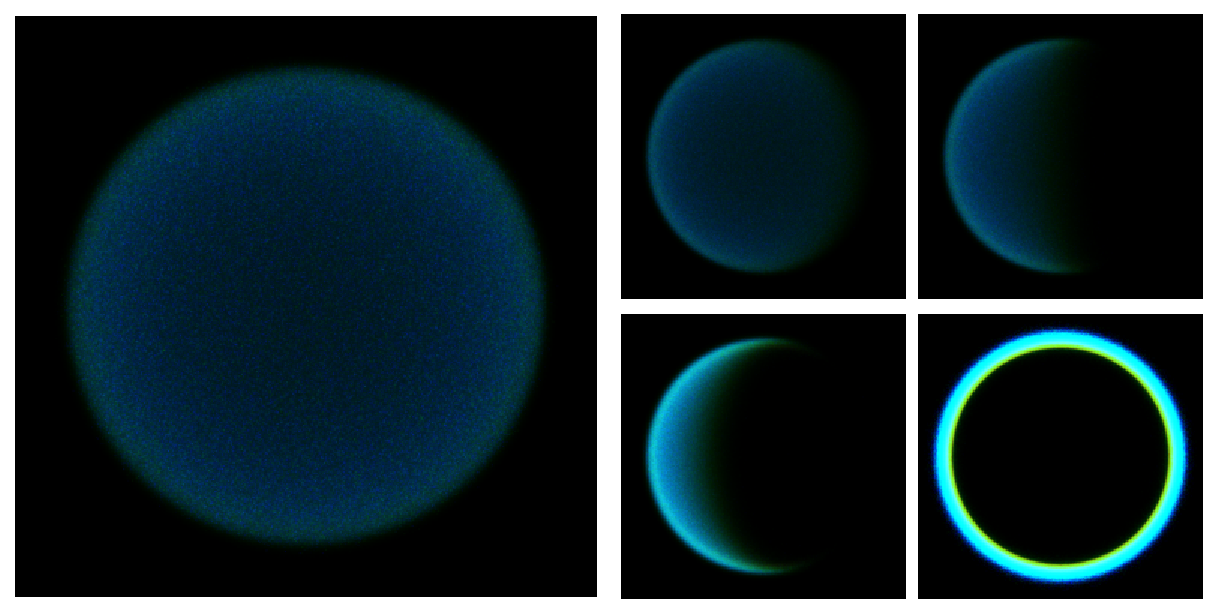
\includegraphics[scale = 0.4]{LambertianSimA0.pdf}

\centering

\caption{SRTC++ Simulation results for a Lambertian Titan with 0.0 surface albedo, colored with 5, 2, and 1.3 $\mu$m mapped to red, green, and blue, respectively. The left image is viewed at 0$^{\circ}$ phase. The right four images are, clockwise from the top left, at 35$^{\circ}$, 90$^{\circ}$, 180$^{\circ}$, and 120$^{\circ}$. \textbf{\color{red}Animating Version: A0.0LambertSimMOVIE.gif\color{black}}}

\label{fig:lamsimA0}

\end{figure}

\begin{figure}[htbp]


\includegraphics[scale = 0.4]{LambertianSim.pdf}

\centering

\caption{SRTC++ Simulation results for a Lambertian Titan with 0.1 surface albedo, colored with 5, 2, and 1.3 $\mu$m mapped to red, green, and blue, respectively. The left image is viewed at 0$^{\circ}$ phase. The right four images are, clockwise from the top left, at 35$^{\circ}$, 90$^{\circ}$, 180$^{\circ}$, and 120$^{\circ}$. \textbf{\color{red}Animating Version: A0.1LambertSimMOVIE.gif\color{black}}}

\label{fig:lamsimA1}

\end{figure}

The simulations are largely as expected for a Lambertian sphere obscured by a thick atmosphere. \cite{Pont2007} shows what a Lambertian sphere should look like without an atmosphere in their Figure 9, and our 0.0 albedo simulation shows us the effect of the atmosphere without any signal coming from the surface. Both atmospheric and surface effects should be active in the 0.1 albedo simulation, and that is precisely what we see in the directly illuminated view: a flat greenish center where there's minimal atmospheric influence that slowly fades off as the emission angle becomes steeper, at which point the atmosphere takes over with its bluish hue.

The coloration is entirely due to atmospheric effects; bluer light is scattered by atmospheric haze more readily than redder light. In the raw data, the blue channel is the largest even in the center at 0.1 albedo. It is merely the choice of color balancing that gives Titan its greenish hue, a sensible choice as it allows us to readily identify places with more surface signal than atmospheric. The center of the disc, when viewed from head-on, is rather uniform with little variation, as expected.

Views other than at zero phase also behave as expected; the limb is atmospherically dominated, becoming bluer. Light is more likely to be forward scattered than backscattered in Titan's atmosphere \citep{GarcaMuoz2017, Cooper2025}, so the closer the Sun gets to behind Titan, the brighter the limb becomes. A Lambertian surface without an atmosphere would have no light coming from anywhere that was not directly illuminated, but we see a small amount of light from beyond the terminator due to atmospheric scattering.

We can also see the shadow Titan casts on its own atmosphere in the profile views as the signal is abruptly diminished near the top and bottom of the moon, but the atmosphere above this shadow remains brightly illuminated. This effect happens on Earth as well and is what causes the colors of twilight \citep{Lynch2004}.

Notably, the ``eclipse'' view at 180$^{\circ}$ phase is functionally identical in all simulations, which it should be as the surface has little influence on the signal at this viewing geometry. There is most certainly interesting science to be done with the simulation at this angle to probe the atmosphere, but such investigations are beyond the scope of this paper.

The simulation results appear slightly grainy due to the Monte-Carlo nature of SRTC++. If we were to run the simulation for longer, the S/N (signal-to-noise ratio) would increase, and the overall image result would become smoother. We deem this unnecessary for our current work, as we will be binning and averaging much of the noise away shortly.

We ultimately seek to compare these simulations with real data. While we can qualitatively see that real Titan images have similar coloration and limb effects \citep{Barnes2005}, the fact that real Titan has numerous different terrain types interferes with any more robust conclusions. Thus, we transform the simulations to present their data based on viewing geometry information, rather than direct visual information. The transformed simulations can, given a specific viewing geometry, describe how a Lambertian Titan would appear at that geometry, which can then be compared to real data. These simulations are effectively transformed into numerical bidirectional reflectance distribution functions (BRDFs).

To construct these transformed simulations, every spectel is sorted into bins based on viewing geometry, and then we average their values. The bins are separated by 5$^{\circ}$ increments in incidence, emission, and azimuth angle, defined as shown in Figure \ref{fig:displaylabel}, with 0$^{\circ}$ azimuth being the forward-scattering direction, and 180$^{\circ}$ being backscattering. This process increases the S/N for combined spectels, addressing the aforementioned "grainy" nature of the simulations.

\begin{figure}[htbp]


\includegraphics[scale = 0.55]{VGDisplayLabel.pdf}

\centering

\caption{Viewing geometry angles used in this paper. The incidence angle is represented by ``i'', the emission angle by ``e'', and the azimuth angle by ``$\phi$''. The arrows trace out a path from the sun (yellow circle) to some arbitrary spot on Titan's surface to a detector (purple diamond). Diagrams modeled after this one appear in future figures to give context for the data.}

\label{fig:displaylabel}

\end{figure}

Notably, our transformed simulations have only three angles, while more traditional BRDFs have four. We do not treat topographic changes in a surface, as such information is very context dependent, so we can safely assume that the sun is always coming in from the same relative direction, removing the need to keep track of the fourth viewing angle. As such, we will call these transformed simulations restricted BRDFs from here on out. This choice also makes it easier to determine when backscattering or forward-scattering is occurring, key indicators of non-Lambertian behavior.

We also differ from traditional BRDFs in another way: the atmospheric contributions are retained. We are not measuring the actual response of the surface to light; we are measuring the apparent response as observed from outside Titan, including all atmospheric effects.

With 3 different albedos and 8 wavelengths, we have a total of 24 restricted BRDFs ready to be compared with other restricted BRDFs compiled from real VIMS data.

\section{Observations and Data} \label{sec:observe}

Cassini performed 127 close flybys of Titan during its mission \citep{Seal2017}, and most of those flybys have observations from Cassini VIMS. Viewing geometries on any single flyby are generally limited in scope, as the spacecraft itself could only examine geometries it personally encountered. Thus, in order to gain a proper understanding of the surface of Titan at a wide range of viewing geometries, we use observations from as many flybys as possible.

The primary obstacle in properly using all the data is the sheer quantity: 127 flybys, tens of thousands of individual observations, and in each of those hundreds of pixels, with 256 spectels each. If we wish to make a single global model, this would not be an issue, as an algorithm could easily ingest everything. However, simple inspection of VIMS images reveals that different terrains have different albedos, and our simulations in Figures \ref{fig:lamsimA0} and \ref{fig:lamsimA1} clearly show how much the appearance of the surface changes with albedo. Averaging all terrain types together could smooth out non-Lambertian behavior, or allow a single non-Lambertian terrain type to contaminate all the others.

As such, we focus our analysis on terrain types. We primarily investigate the equatorial regions between 30$^{\circ}$ and -30$^{\circ}$ latitude since that's where Huygens sampled the atmosphere \citep{Tomasko2008}, making this region the best characterized. We also want terrain types that are examined from a wide variety of viewing geometries with a large number of reliable observations. We judge that only Titan's equatorial dunes meet all these criteria. (We had considered the equatorial bright terrain as well, but the results we obtain from it are inconsistent and unreliable.) To gather the relevant data, we create a raster mask of Titan's equatorial dunes in Figure \ref{fig:dunemask} at a resolution of one pixel per degree on Titan's surface; 181 in latitude and 360 in longitude.

\begin{figure*}[tbp]

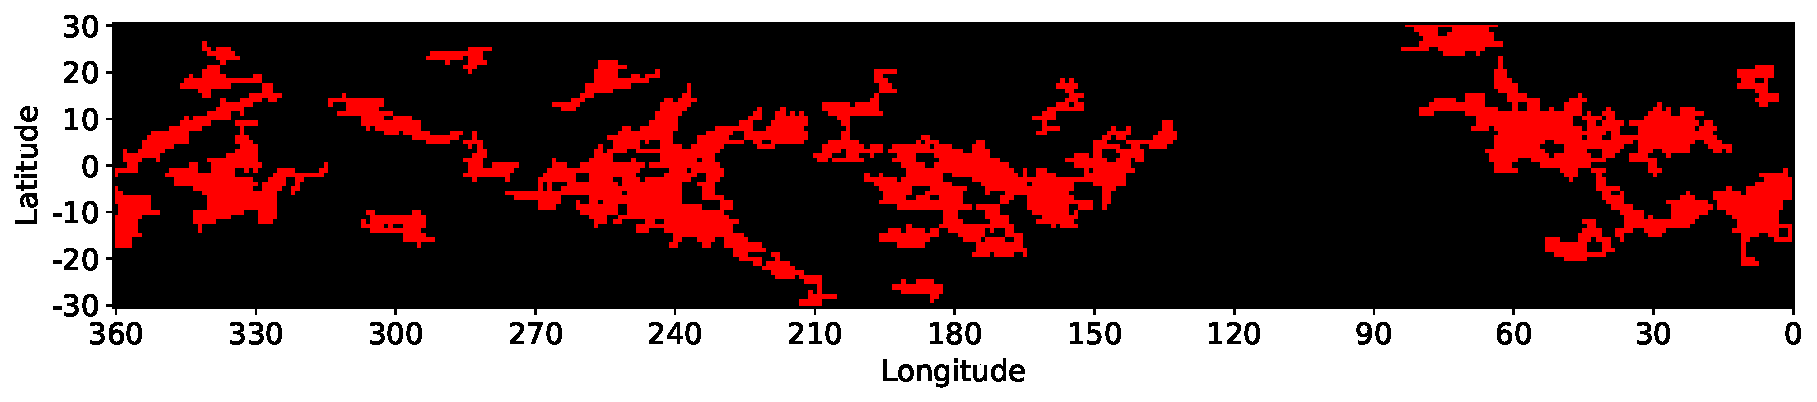
\includegraphics[scale = 0.5]{TitanSurfaceMaskDunes.pdf}

\centering

\caption{Titan equatorial surface terrain mask for dunes, as informed by \cite{Lopes2020} mixed with VIMS observations. The red pixels are dunes; black pixels are everything else. Almost all of the dunes on Titan are included in this mask, though there are a few small regions outside the 30$^{\circ}$ and -30$^{\circ}$ latitude boundaries.}

\label{fig:dunemask}

\end{figure*}

The creation of the mask begins with the Titan terrain map created by \cite{Lopes2020} using radar data. VIMS observations, which are taken in IR, often don't match the radar observations \citep{Soderblom2007}, but tend to agree in the bulk of major features. Most notably (and importantly for this paper), the dunes have good agreement on a global scale.

VIMS observations come in files called cubes. Our investigation procedure for these cubes begins with a basic database search; in our specific case, we look for any cubes that have pixels in the equatorial regions between 30$^{\circ}$ and -30$^{\circ}$ latitude, and also have pixels of 25 km ground resolution or finer. The database we use has already filtered out clearly erroneous files, as well as so-called ``noodle'' images which are only a handful of pixels in diameter. The cubes themselves are calibrated with the standard VIMS pipeline \citep{Barnes2007}.

Each pixel that matches our criteria is put into a list. We then bin spectels within each pixel in the list and create a restricted BRDF out of them in a process identical to that described in Section \ref{sec:mresults}. Unlike many other investigations, we do not subtract off atmospheric contributions, as our simulations include those effects.

There are a few limitations to the created restricted BRDFs. The primary limitation is that bins at certain viewing angles, usually at the extreme ends of allowed values, have no value since Cassini was never in those positions. There is also no check for interfering clouds during the creation process.

Particularly fine-resolution cubes can separate spectral end members that are mixed together in coarser observations and thus are not reflected in the mask, such as a handful of VIMS observations that can see interdune areas \citep{Barnes2008}. These pure spectral endmembers need not match the behavior of the terrain they are surrounded by, and could conceivably offset the final model. The interdune areas are known to vary considerably across Titan \citep{Bonnefoy2016}. Fortunately, the restricted BRDFs created for the dunes exhibit remarkable consistency and order, despite the interdunes' presence. We are unsure precisely why this consistency exists--it could be that a single kind of interdune dominates most of Titan's dunes, and all others are insignificant, making the result orderly. Alternatively, the various interdune types could be drowned out by the sheer amount of data averaging occurring.

We expect that any retrieved albedos from this model will most likely be biased higher than pure dune sands, given the brighter interdunes \citep{Bonnefoy2016}. However, as we are examining the dunes terrain type as a whole, we do not consider this a detriment to any of our results.

In addition to the dunes, we also derive restricted BRDFs for the Huygens landing site, allowing for more direct comparisons to observations made by the Huygens lander \citep{Tomasko2008}. We perform a database search similarly to how we make the other models, but instead of using the mask, we go in manually, cleaning up any situations where the wrong latitude and longitude are obtained due to ephemeris uncertainties that are most likely sourced from within the program SPICE \citep{Anton1999} used to retrieve metadata. This ensures that the data are devoid of any contamination; a caution we only had to exercise since the Huygens landing site is such a small area on the boundary of multiple terrain types.

In order to counteract the lack of observational geometries for both the equatorial dunes and the Huygens landing site, we perform tetrahedral interpolation to fill in as many observation angles as possible in the restricted BRDFs using the PyVista package \citep{Sullivan2019}.

\section{Simulation vs Data Comparison} \label{sec:compare}

\subsection{Huygens Landing Site} \label{sec:huygensC}

We choose to examine the Huygens landing site first as its data set is simpler, covering significantly fewer viewing geometries than the dunes. As three-dimensional data (incidence, emission, and azimtuh angles in this case) are hard to visualize, we opt to plot individual one-dimensional ``skewers'' of the restricted BRDFs at a time, fixing two of the three viewing geometry angles while allowing the third to vary. We create skewers for all restricted BRDFs, be they simulations or real data. We plot select representative skewers of the three simulations and Huygens landing site data in Figures \ref{fig:inciskewer}-\ref{fig:azimskewer}. Each considers a different viewing angle along its x-axis: Figure \ref{fig:inciskewer} showcases the incidence angle at 35$^{\circ}$ emission and 55$^{\circ}$ azimuth, Figure \ref{fig:emisskewer} showcases the emission angle at 35$^{\circ}$ incidence and 50$^{\circ}$ azimuth, and Figure \ref{fig:azimskewer} showcases the azimuth angle at 35$^{\circ}$ incidence and 30$^{\circ}$ emission.

\begin{figure*}[htbp]

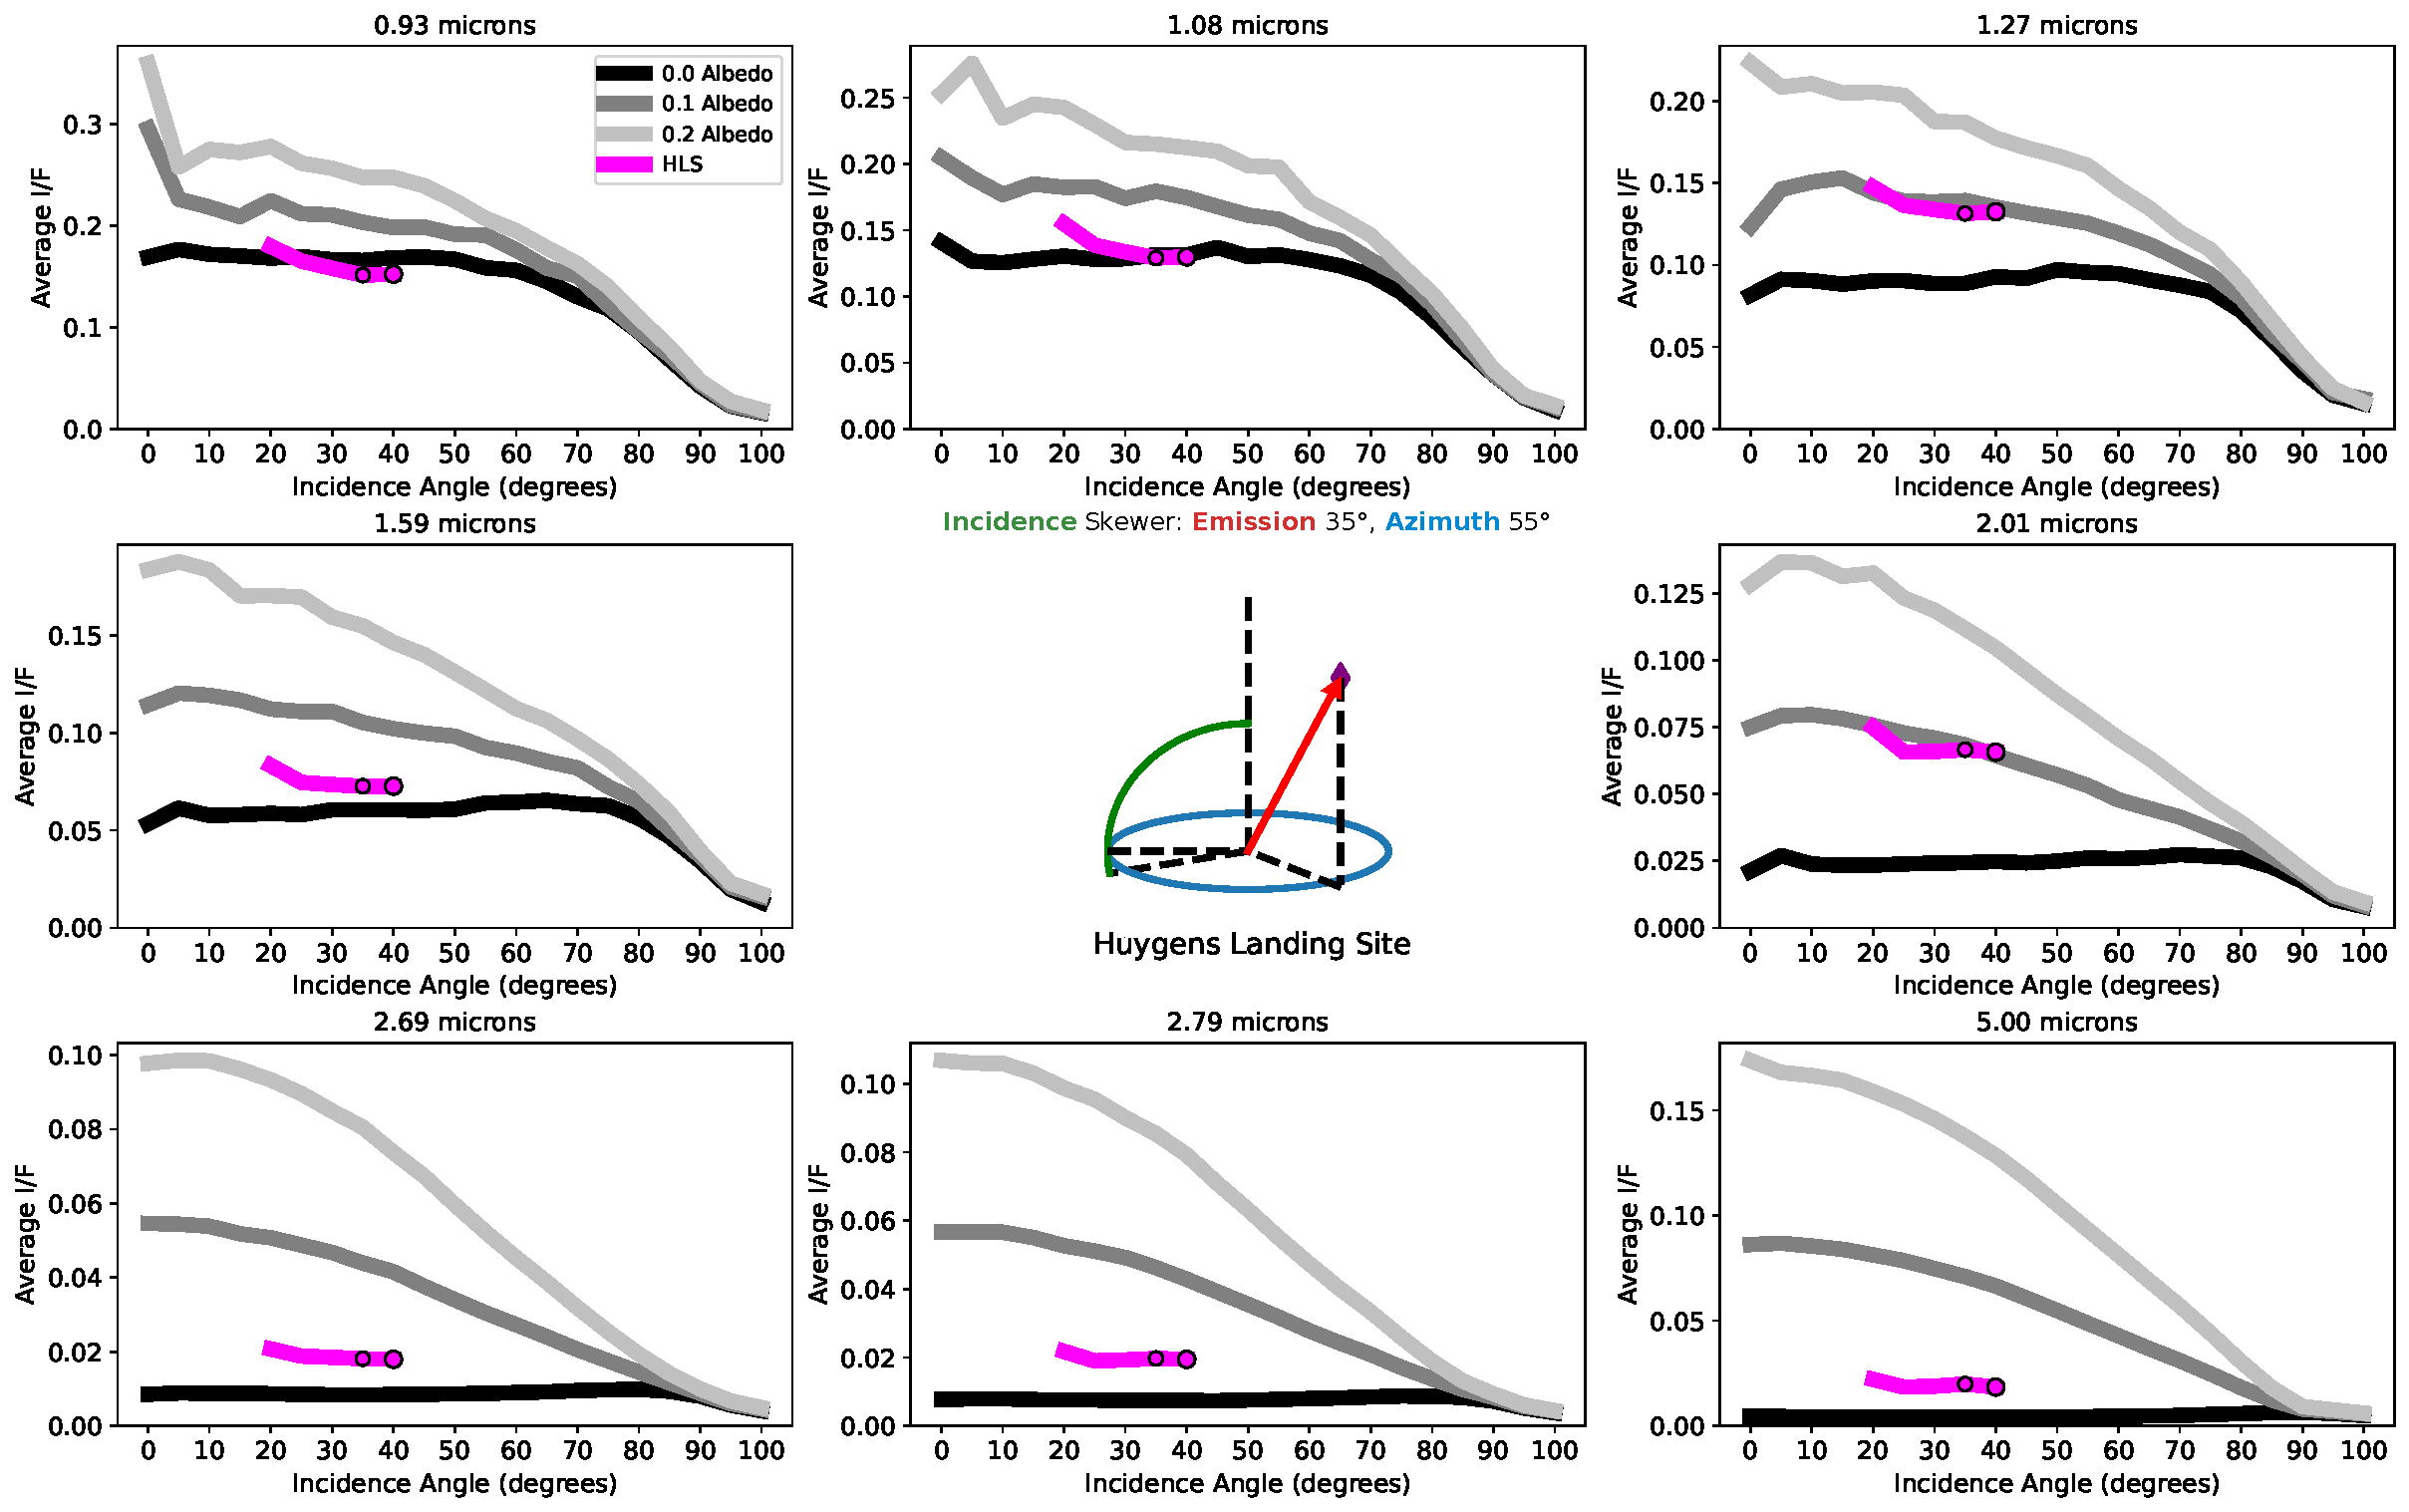
\includegraphics[scale = 0.4]{HLSInciSkewer.pdf}

\centering

\caption{Average I/F (radiance factor) incidence angle skewers for the Huygens landing site with emission angle fixed at 35$^{\circ}$ and azimuth angle at 55$^{\circ}$. All eight wavelengths are arranged from shortest to longest, starting from the top left corner. Simulation lines are monochromatic; the Huygens landing site data are pink. Bins with direct Huygens landing site observations have dots plotted over the lines, with larger dots indicating more observations. Bins on the Huygens landing site lines without dots are interpolated values. Note that the vertical axis scale is different for each wavelength. The central area is occupied by a geometry diagram illustrating the specific geometry bins considered for these skewers. All considered incidence angles are represented by a green arc, while the specific emission and azimuth are portrayed by the red vector and the dotted lines that give perspective relative to a blue azimuthal ring representing the surface.}

\label{fig:inciskewer}

\end{figure*}

\begin{figure*}[htbp]

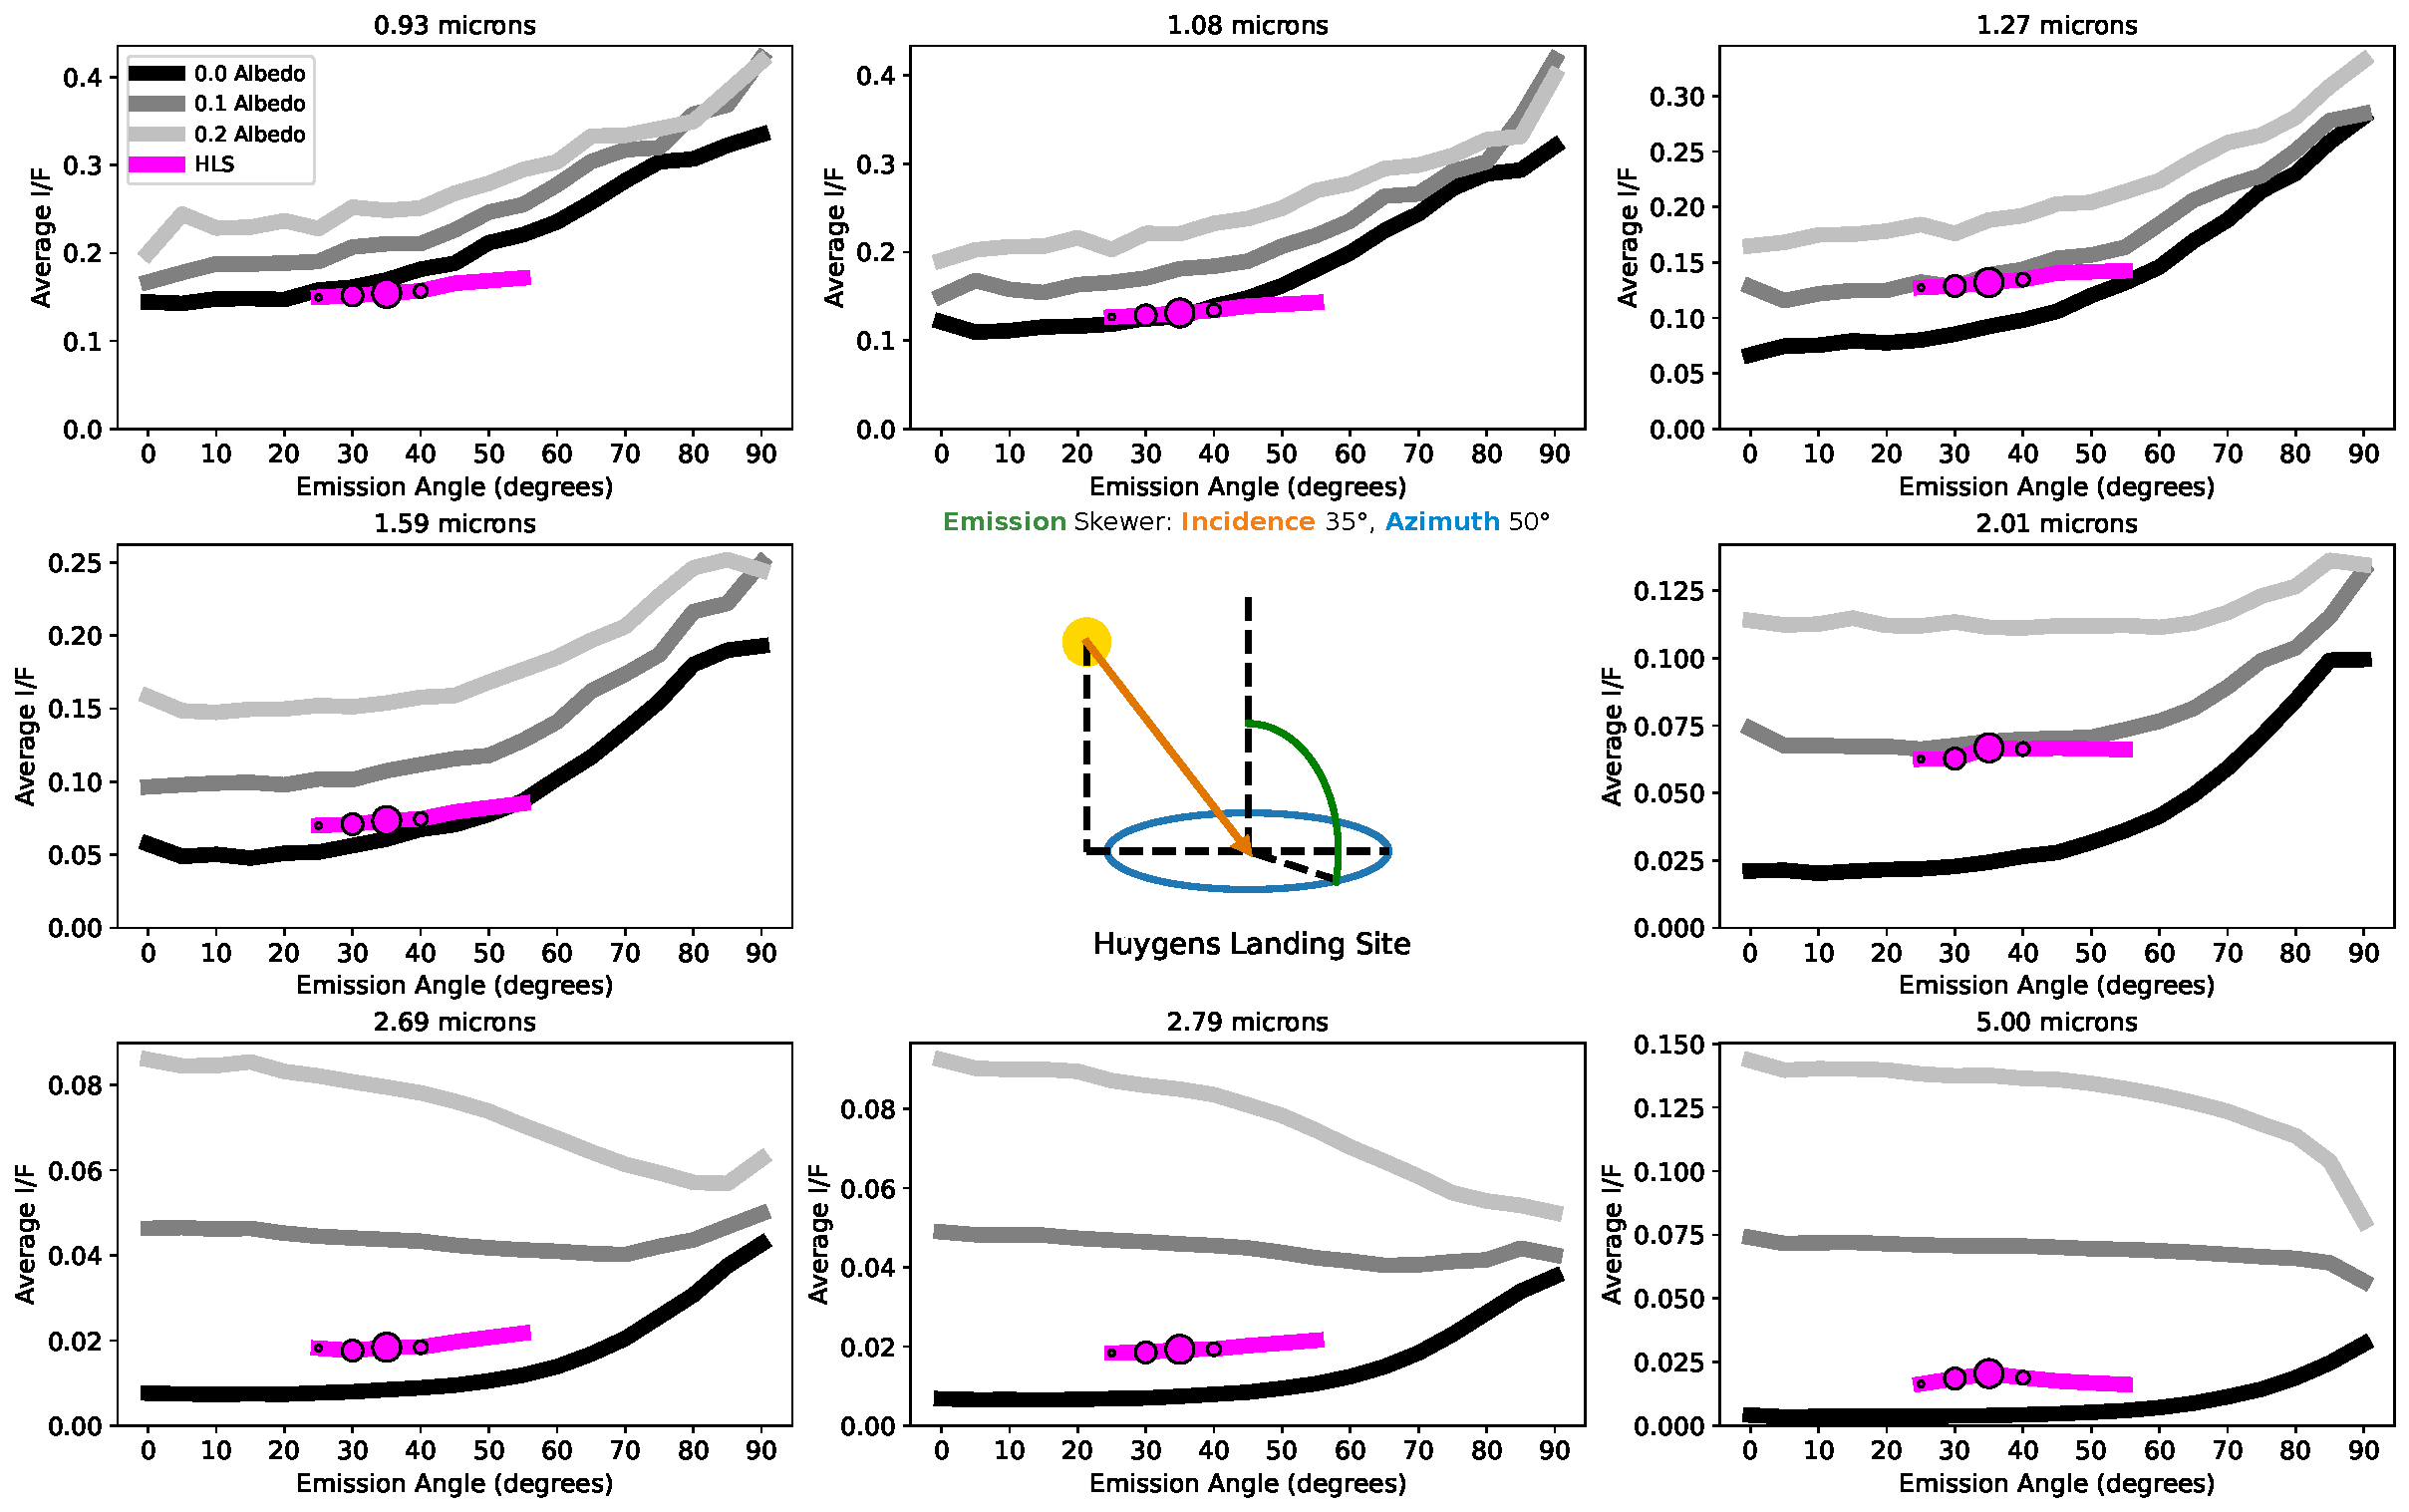
\includegraphics[scale = 0.4]{HLSEmisSkewer.pdf}

\centering

\caption{Average I/F emission angle skewers for the Huygens landing site with incidence angle fixed at 35$^{\circ}$ and azimuth angle at 50$^{\circ}$. All eight wavelengths are arranged from shortest to longest, starting from the top left corner. Simulation lines are monochromatic; the Huygens landing site data are pink. Bins with direct Huygens landing site observations have dots plotted over the lines, with larger dots indicating more observations. Bins on the Huygens landing site lines without dots are interpolated values. Note that the vertical axis scale is different for each wavelength. The central area is occupied by a geometry diagram illustrating the specific geometry bins considered for these skewers. All considered emission angles are represented by a green arc, which is tilted at the specific azimuth angle, using a vertical dotted line to give perspective. The orange line represents the incidence angle, or incoming light.}

\label{fig:emisskewer}

\end{figure*}

\begin{figure*}[htbp]

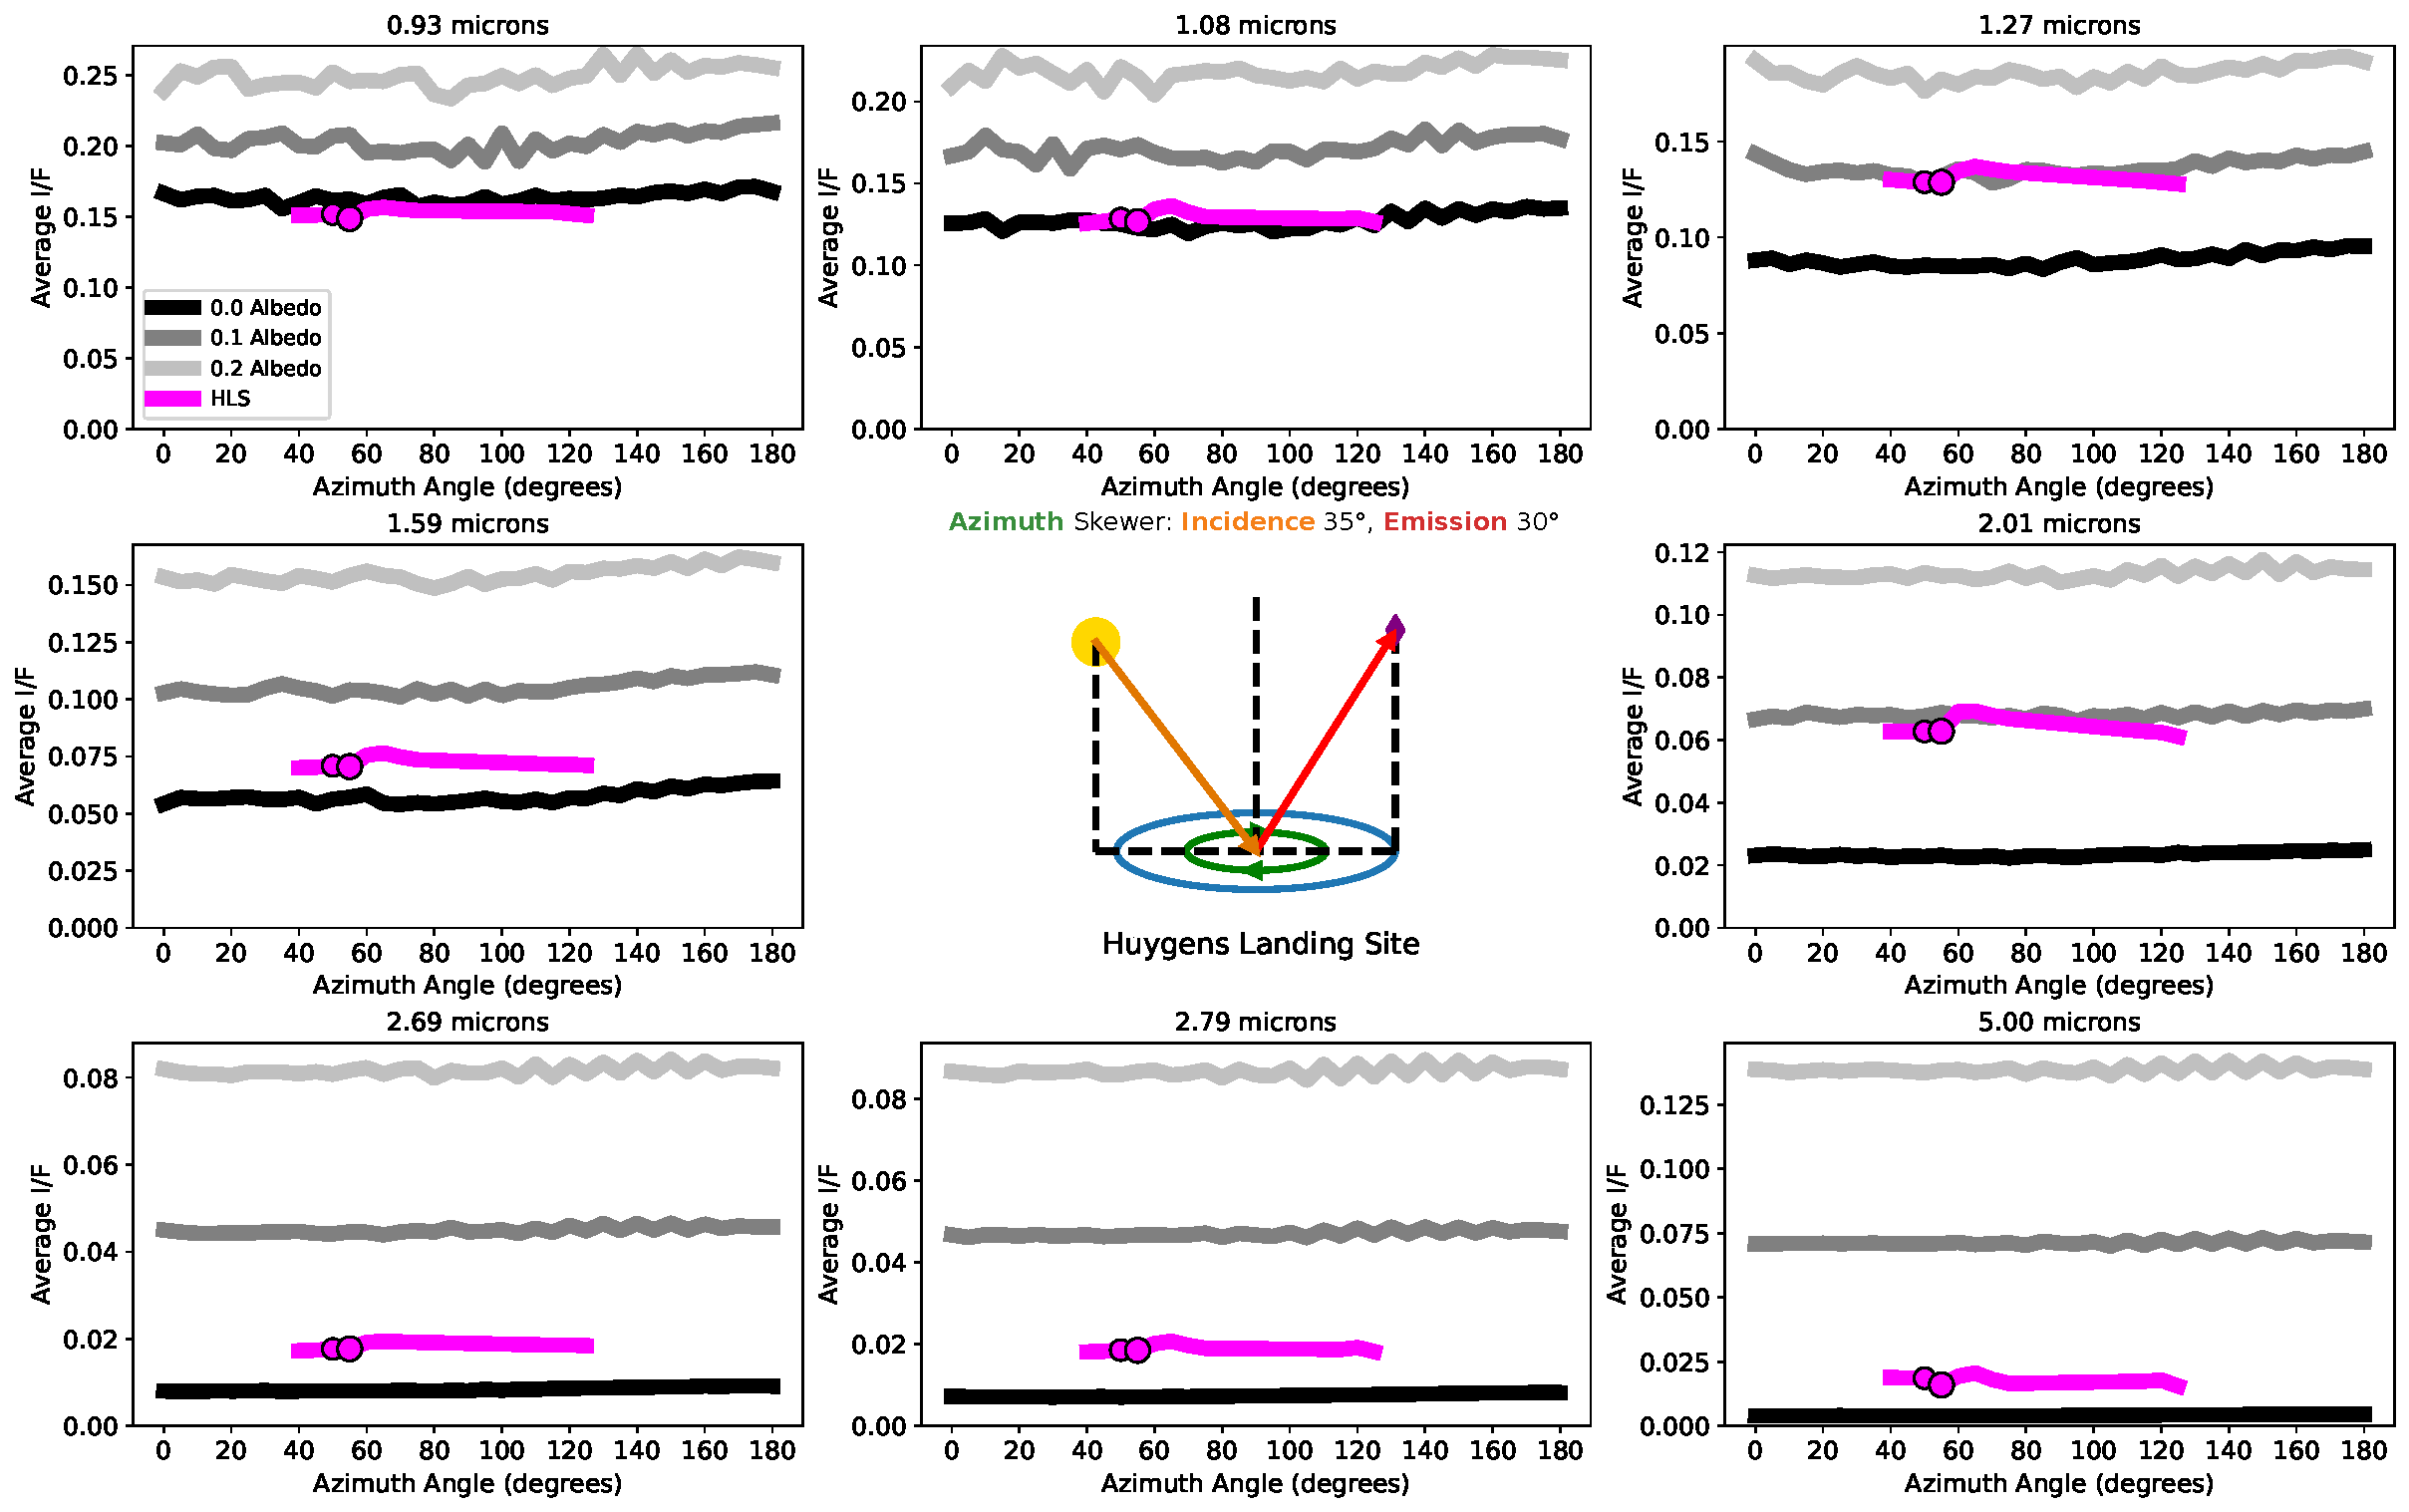
\includegraphics[scale = 0.4]{HLSAzimuthSkewer.pdf}

\centering

\caption{Average I/F azimuth angle skewers for the Huygens landing site with incidence angle fixed at 35$^{\circ}$ and emission angle at 30$^{\circ}$. All eight wavelengths are arranged from shortest to longest, starting from the top left corner. Simulation lines are monochromatic; the Huygens landing site data are pink. Bins with direct Huygens landing site observations have dots plotted over the lines, with larger dots indicating more observations. Bins on the Huygens landing site lines without dots are interpolated values. Note that the vertical axis scale is different for each wavelength. The central area is occupied by a geometry diagram illustrating the specific geometry bins considered for these skewers. All considered azimuth angles are represented by a green circle that coincides with the blue circle representing the surface. The orange and red vectors depict the incidence and emission angles, respectively.}

\label{fig:azimskewer}

\end{figure*}

The simulations naturally extend far beyond where the Huygens landing site was viewed, and it is worth considering their behavior in such regimes. All three skewer types show a distinct shifting of behavior across the various wavelengths. In general, shorter wavelengths show higher I/F (radiance factor) as light traverses through a higher optical depth of highly reflective haze aerosols \citep{EsSayeh2023}, allowing for more scattering events in more directions. Longer wavelengths are usually dimmer, though 5.00 $\mu$m is often slightly brighter than 2.79 $\mu$m.

Incidence skewers almost always have a characteristic pattern, with the three different albedo simulations spread out in I/F at low incidence, lowering in I/F and coming closer together as incidence increases, until at the highest incidences the simulations might as well be indistinguishable from each other. The general incidence behavior is exemplified by Figure \ref{fig:inciskewer}'s skewers at 35$^{\circ}$ emission and 55$^{\circ}$ azimuth.

Emission skewers follow a similar but inverted pattern to the incidence skewers and see more variability between the different windows. As a general rule, lower emission angles have the different albedo simulations sperad out with relatively low I/F, and high emission has the simulations closer together with relatively high I/F. At the shortest wavelengths, there is minimal difference between the simulations' I/F, but I/F still rises with emission. The longer wavelengths start to deviate from the pattern where the 0.2 albedo simulation trends downward in I/F with higher emission, while 0.1 lies flat, and only 0.0 rises. 5 $\mu$m almost always behaves this way. The other long wavelengths change behavior based on the specific viewing geometry. Figure \ref{fig:emisskewer}'s emission skewers at 35$^{\circ}$ emission and 50$^{\circ}$ azimuth exemplify this curious long wavelength behavior.

Azimuth skewers tend to be mostly flat in the simulation results, as can be seen in Figure \ref{fig:azimskewer}'s skewers at 35$^{\circ}$ incidence and 30$^{\circ}$ emission. Azimuth skewer behavior does change when both incidence and emission are somewhat large, as forward-scattering behavior begins to be predicted.

Across these three figures, only a small selection of the total three-dimensional histogram is shown; behavior can change significantly when skewering at different incidence, emission, or azimuth angles, though the transitions are always relatively smooth. These particular skewers were chosen because they have the best Huygens landing site data visualizations.

The Huygens landing site data are well behaved for the most part, interpolating smoothly and forming lines that correspond rather well to the simulations. In 1.27 and 2.01 $\mu$m, the data line up almost perfectly with the 0.1 albedo simulation. 0.93 and 1.59 $\mu$m have around 0.05 albedo, and the three longest windows have about 0.03 albedo.

1.08 $\mu$m hugs the 0.0 albedo line, and of all the wavelengths, it shows the largest deviation from parallel to the simulation, most notable in Figure \ref{fig:inciskewer}'s incidence skewers at 35$^{\circ}$ emission and 55$^{\circ}$ azimuth. We are unsure why 1.08 $\mu$m in particular deviates from the simulated curve because we expect 0.93 and 1.08 $\mu$m data to act similarly due to the large atmospheric contributions and unmodeled Rayleigh scattering at these shorter wavelengths.

Even considering 1.08 $\mu$m's quirks, the Huygens landing site appears consistent with a Lambertian surface in the limited viewing geometries to which we have access, which admittedly are not very many. We chose the best skewers we could for Figures \ref{fig:inciskewer}-\ref{fig:azimskewer}, and even the azimuth skewers only cover about a third of the available values. Cassini's observations of the Huygens landing site do not probe the higher incidence and emission angles, and the extremes aren't even approached. Thus, we move to a much larger data set: the equatorial dunes.

\subsection{Equatorial Dunes} \label{sec:dunesC}

Similarly to the Huygens landing site data, we plot three representative one-dimensional skewer sets for the dunes, one for each of the observation angles. Each considers a different viewing angle along its x-axis: Figure \ref{fig:dunesinciskewer} showcases the incidence angle at 5$^{\circ}$ emission and 50$^{\circ}$ azimuth, Figure \ref{fig:dunesemisskewer} showcases the emission angle at 75$^{\circ}$ incidence and 175$^{\circ}$ azimuth, and Figure \ref{fig:dunesazimskewer} showcases the azimuth angle at 40$^{\circ}$ incidence and 30$^{\circ}$ emission.

\begin{figure*}[htbp]

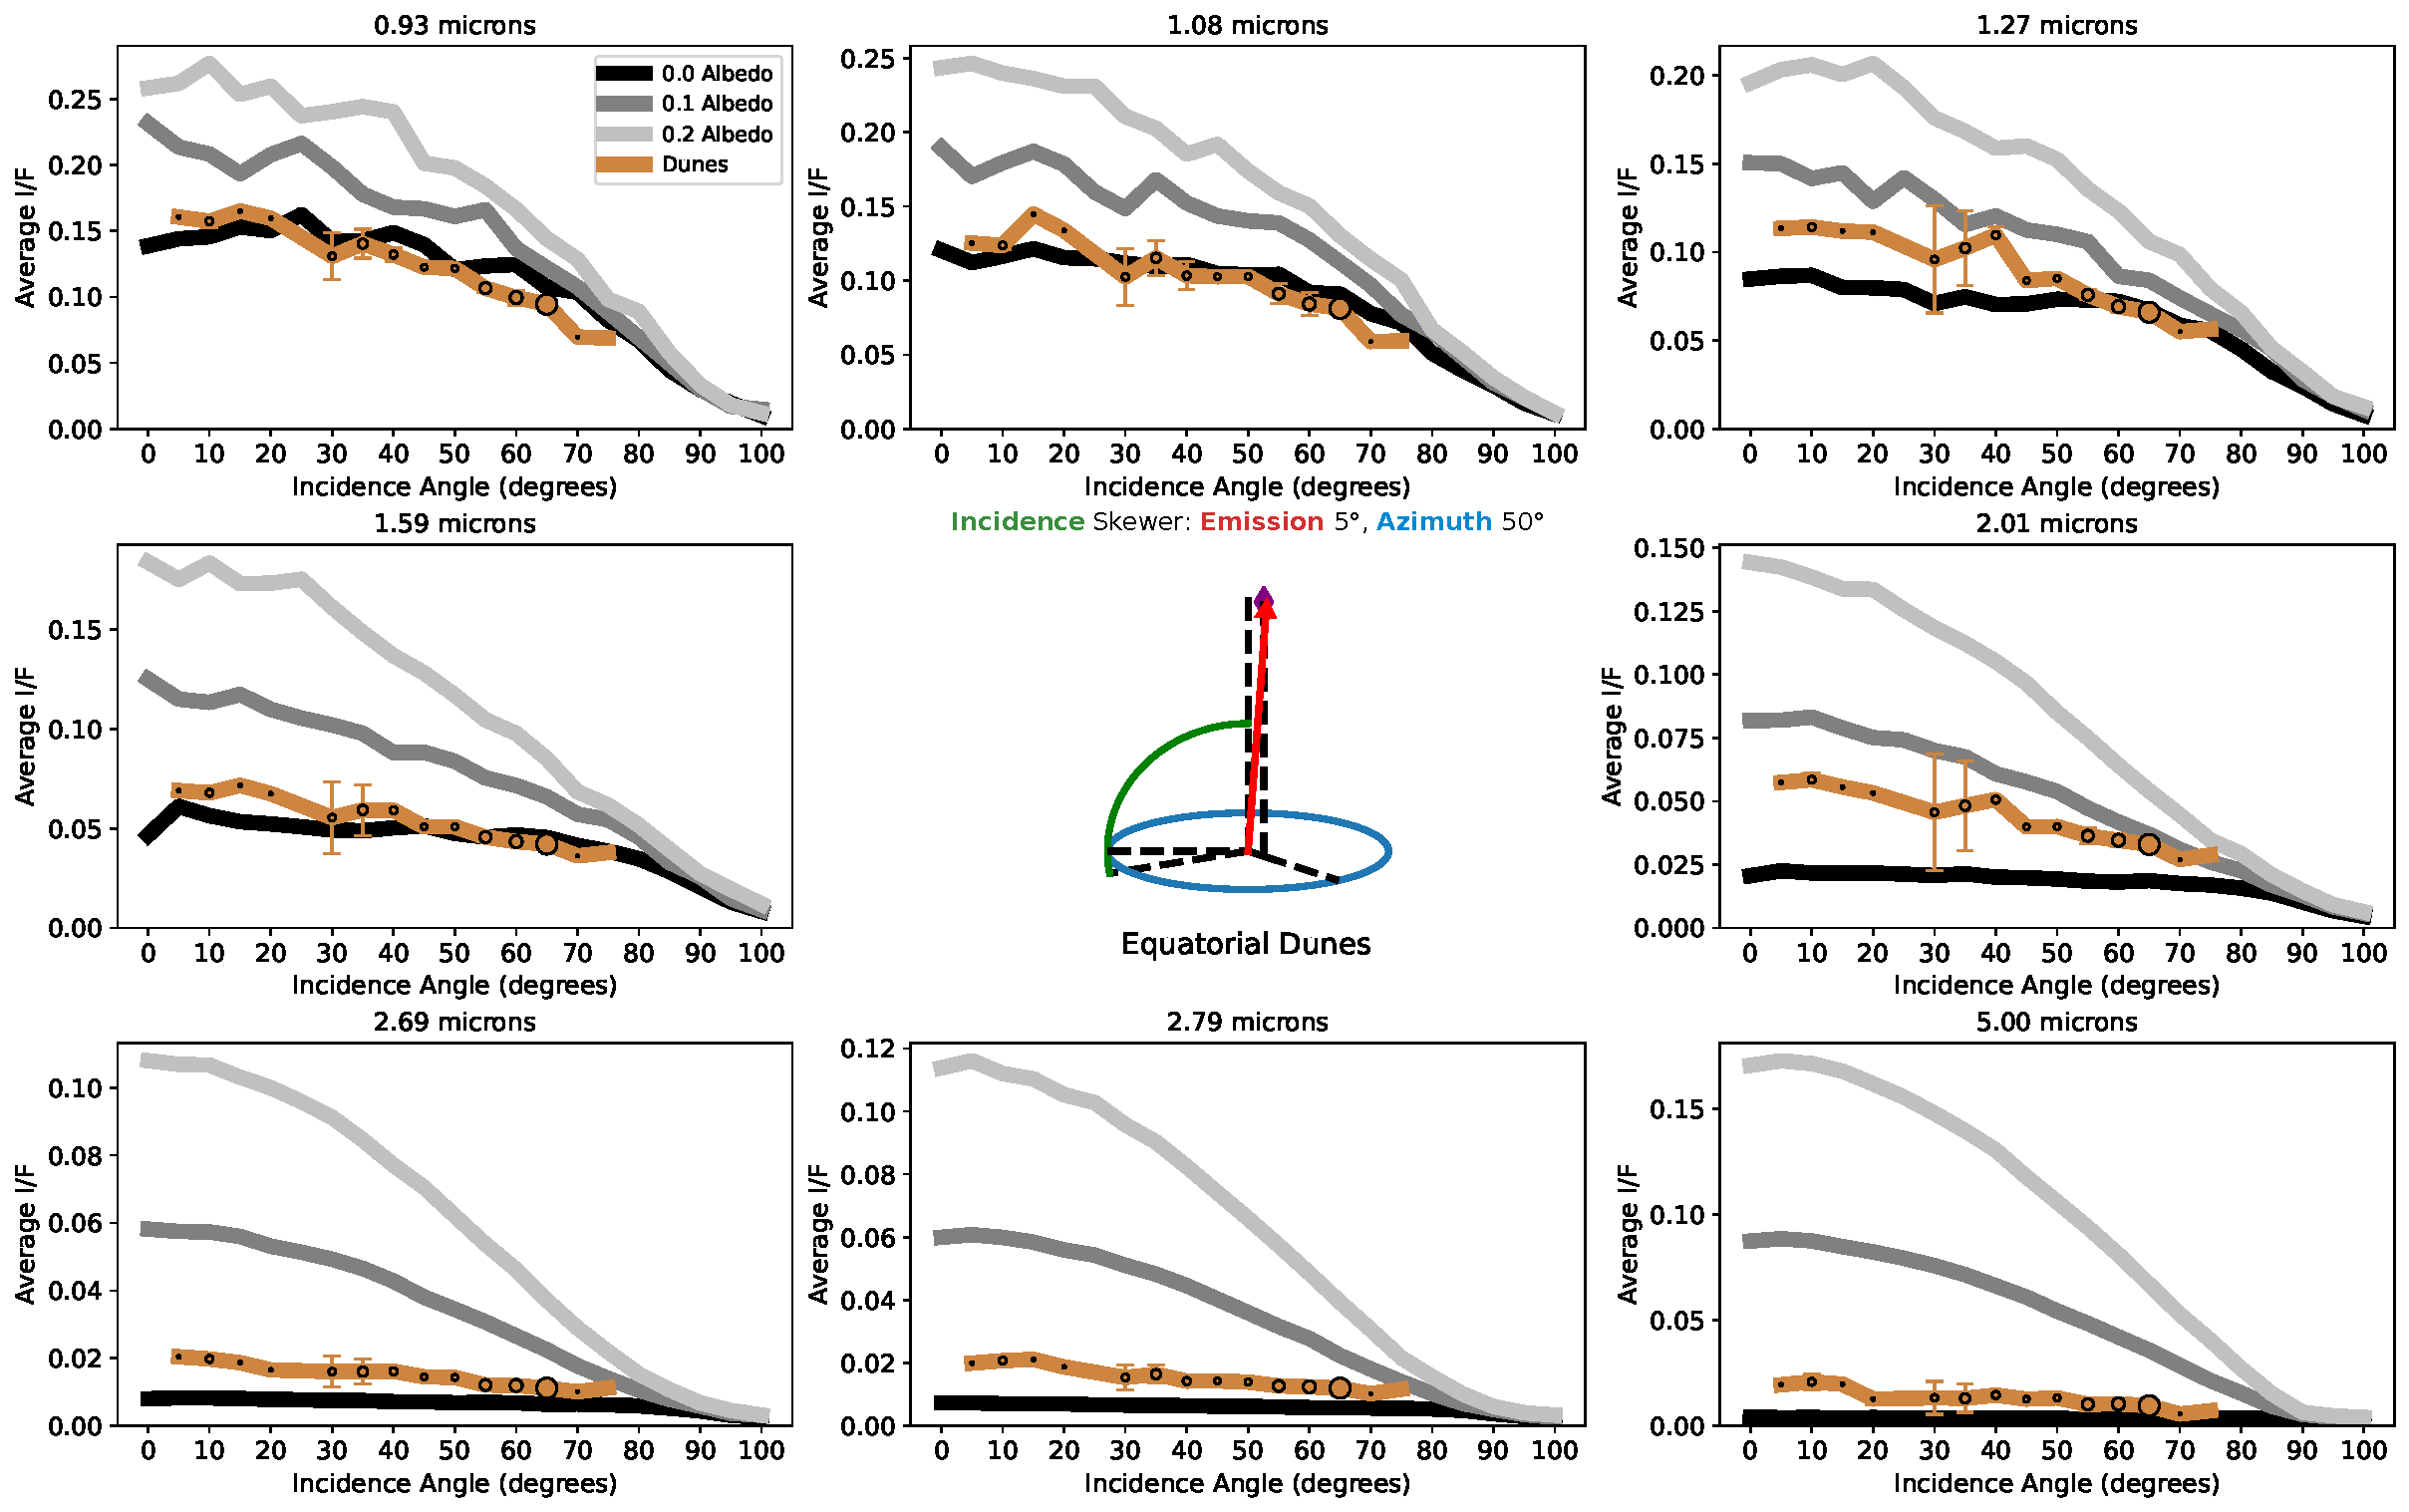
\includegraphics[scale = 0.4]{DunesInciSkewerNEW.pdf}

\centering

\caption{Average I/F incidence angle skewers for the equatorial dunes with emission angle fixed at 5$^{\circ}$ and azimuth angle at 50$^{\circ}$. All eight wavelengths are arranged from shortest to longest, starting from the top left corner. Simulation lines are monochromatic, and the equatorial dunes data are brown. Bins with direct dunes observations have dots plotted over the lines, with larger dots indicating more observations. Segments on the dunes lines without dots are interpolated values. Error bars are made from each noninterpolated bin's standard deviation; most errors are too small to be seen. Note that the vertical axis scale is different for each wavelength. The central area is occupied by a geometry diagram illustrating the specific geometry bins considered for these skewers. All considered incidence angles are represented by a green arc, while the specific emission and azimuth are portrayed by the red vector and the dotted lines that give perspective relative to a blue azimuthal ring representing the surface.}

\label{fig:dunesinciskewer}

\end{figure*}

\begin{figure*}[htbp]

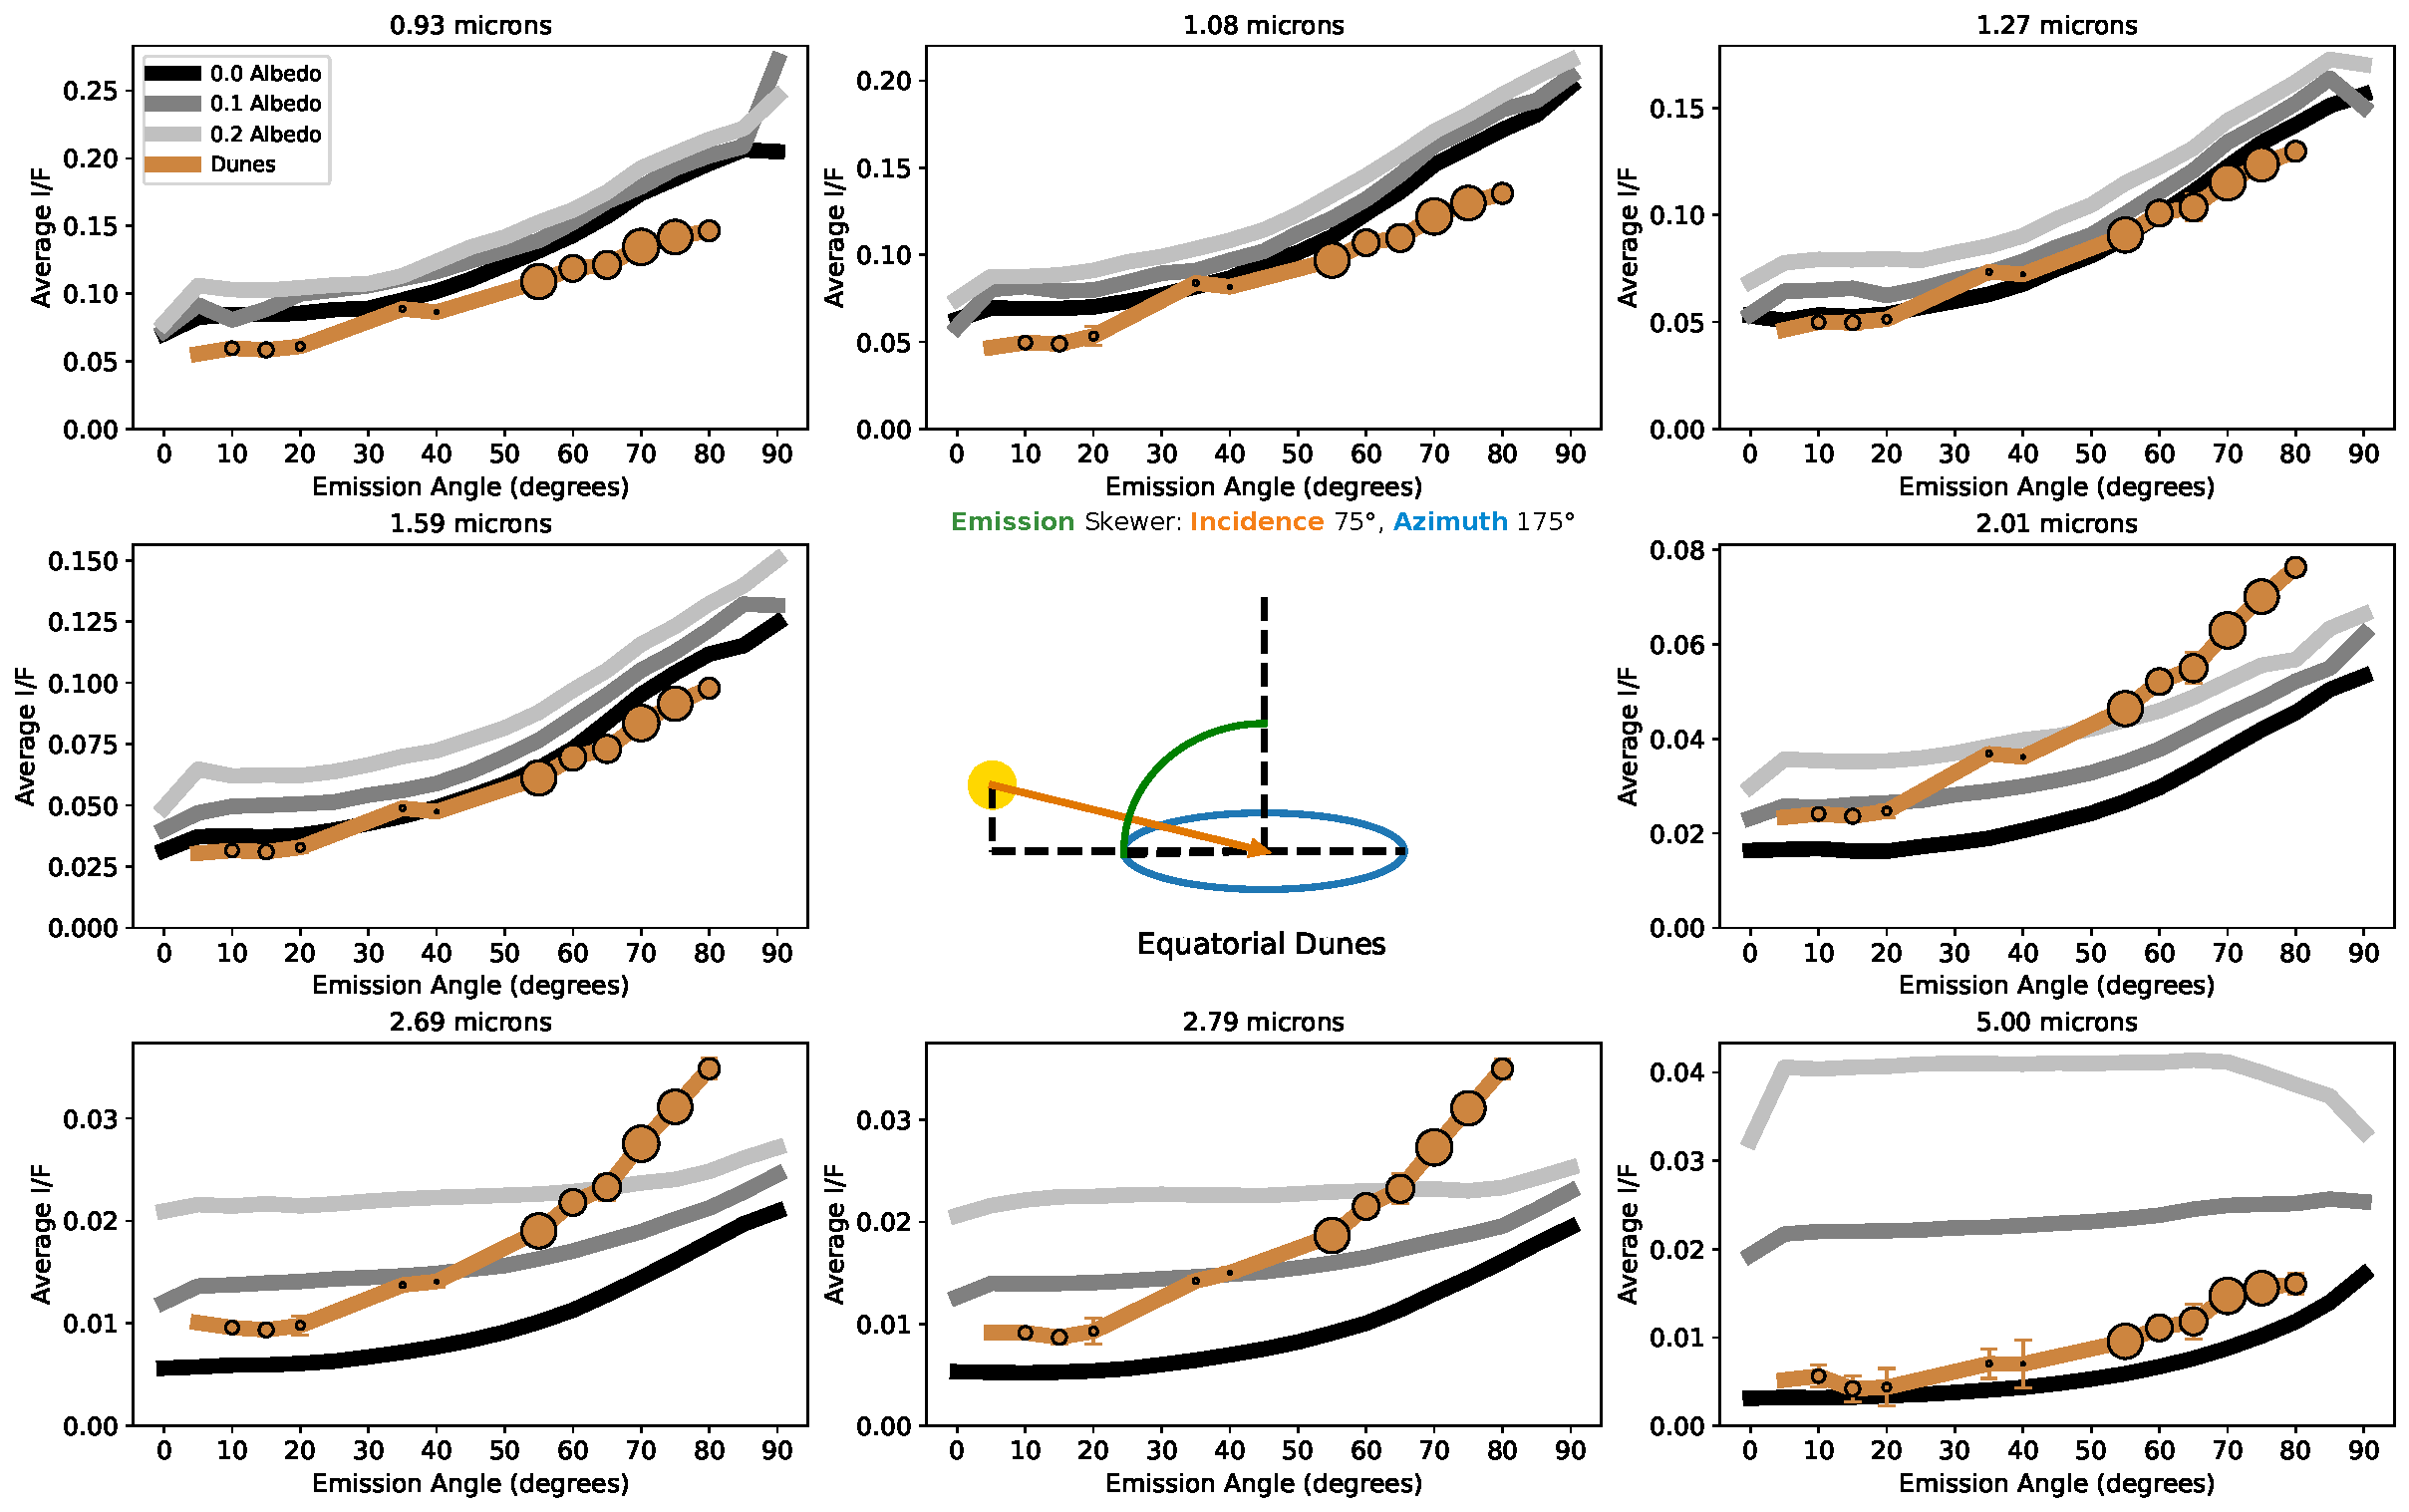
\includegraphics[scale = 0.4]{DunesEmisSkewerNEW.pdf}

\centering

\caption{Average I/F emission angle skewers for the equatorial dunes with incidence angle fixed at 75$^{\circ}$ and azimuth angle at 175$^{\circ}$. All eight wavelengths are arranged from shortest to longest, starting from the top left corner. Simulation lines are monochromatic, and the equatorial dunes data are brown. Bins with direct dunes observations have dots plotted over the lines, with larger dots indicating more observations. Segments on the dunes lines without dots are interpolated values. Error bars are made from each noninterpolated bin's standard deviation; most errors are too small to be seen. Note that the vertical axis scale is different for each wavelength. The central area is occupied by a geometry diagram illustrating the specific geometry bins considered for these skewers. All considered emission angles are represented by a green arc, which is tilted at the specific azimuth angle, using a vertical dotted line to give perspective. The orange line represents the incidence angle, or incoming light.}

\label{fig:dunesemisskewer}

\end{figure*}

\begin{figure*}[htbp]

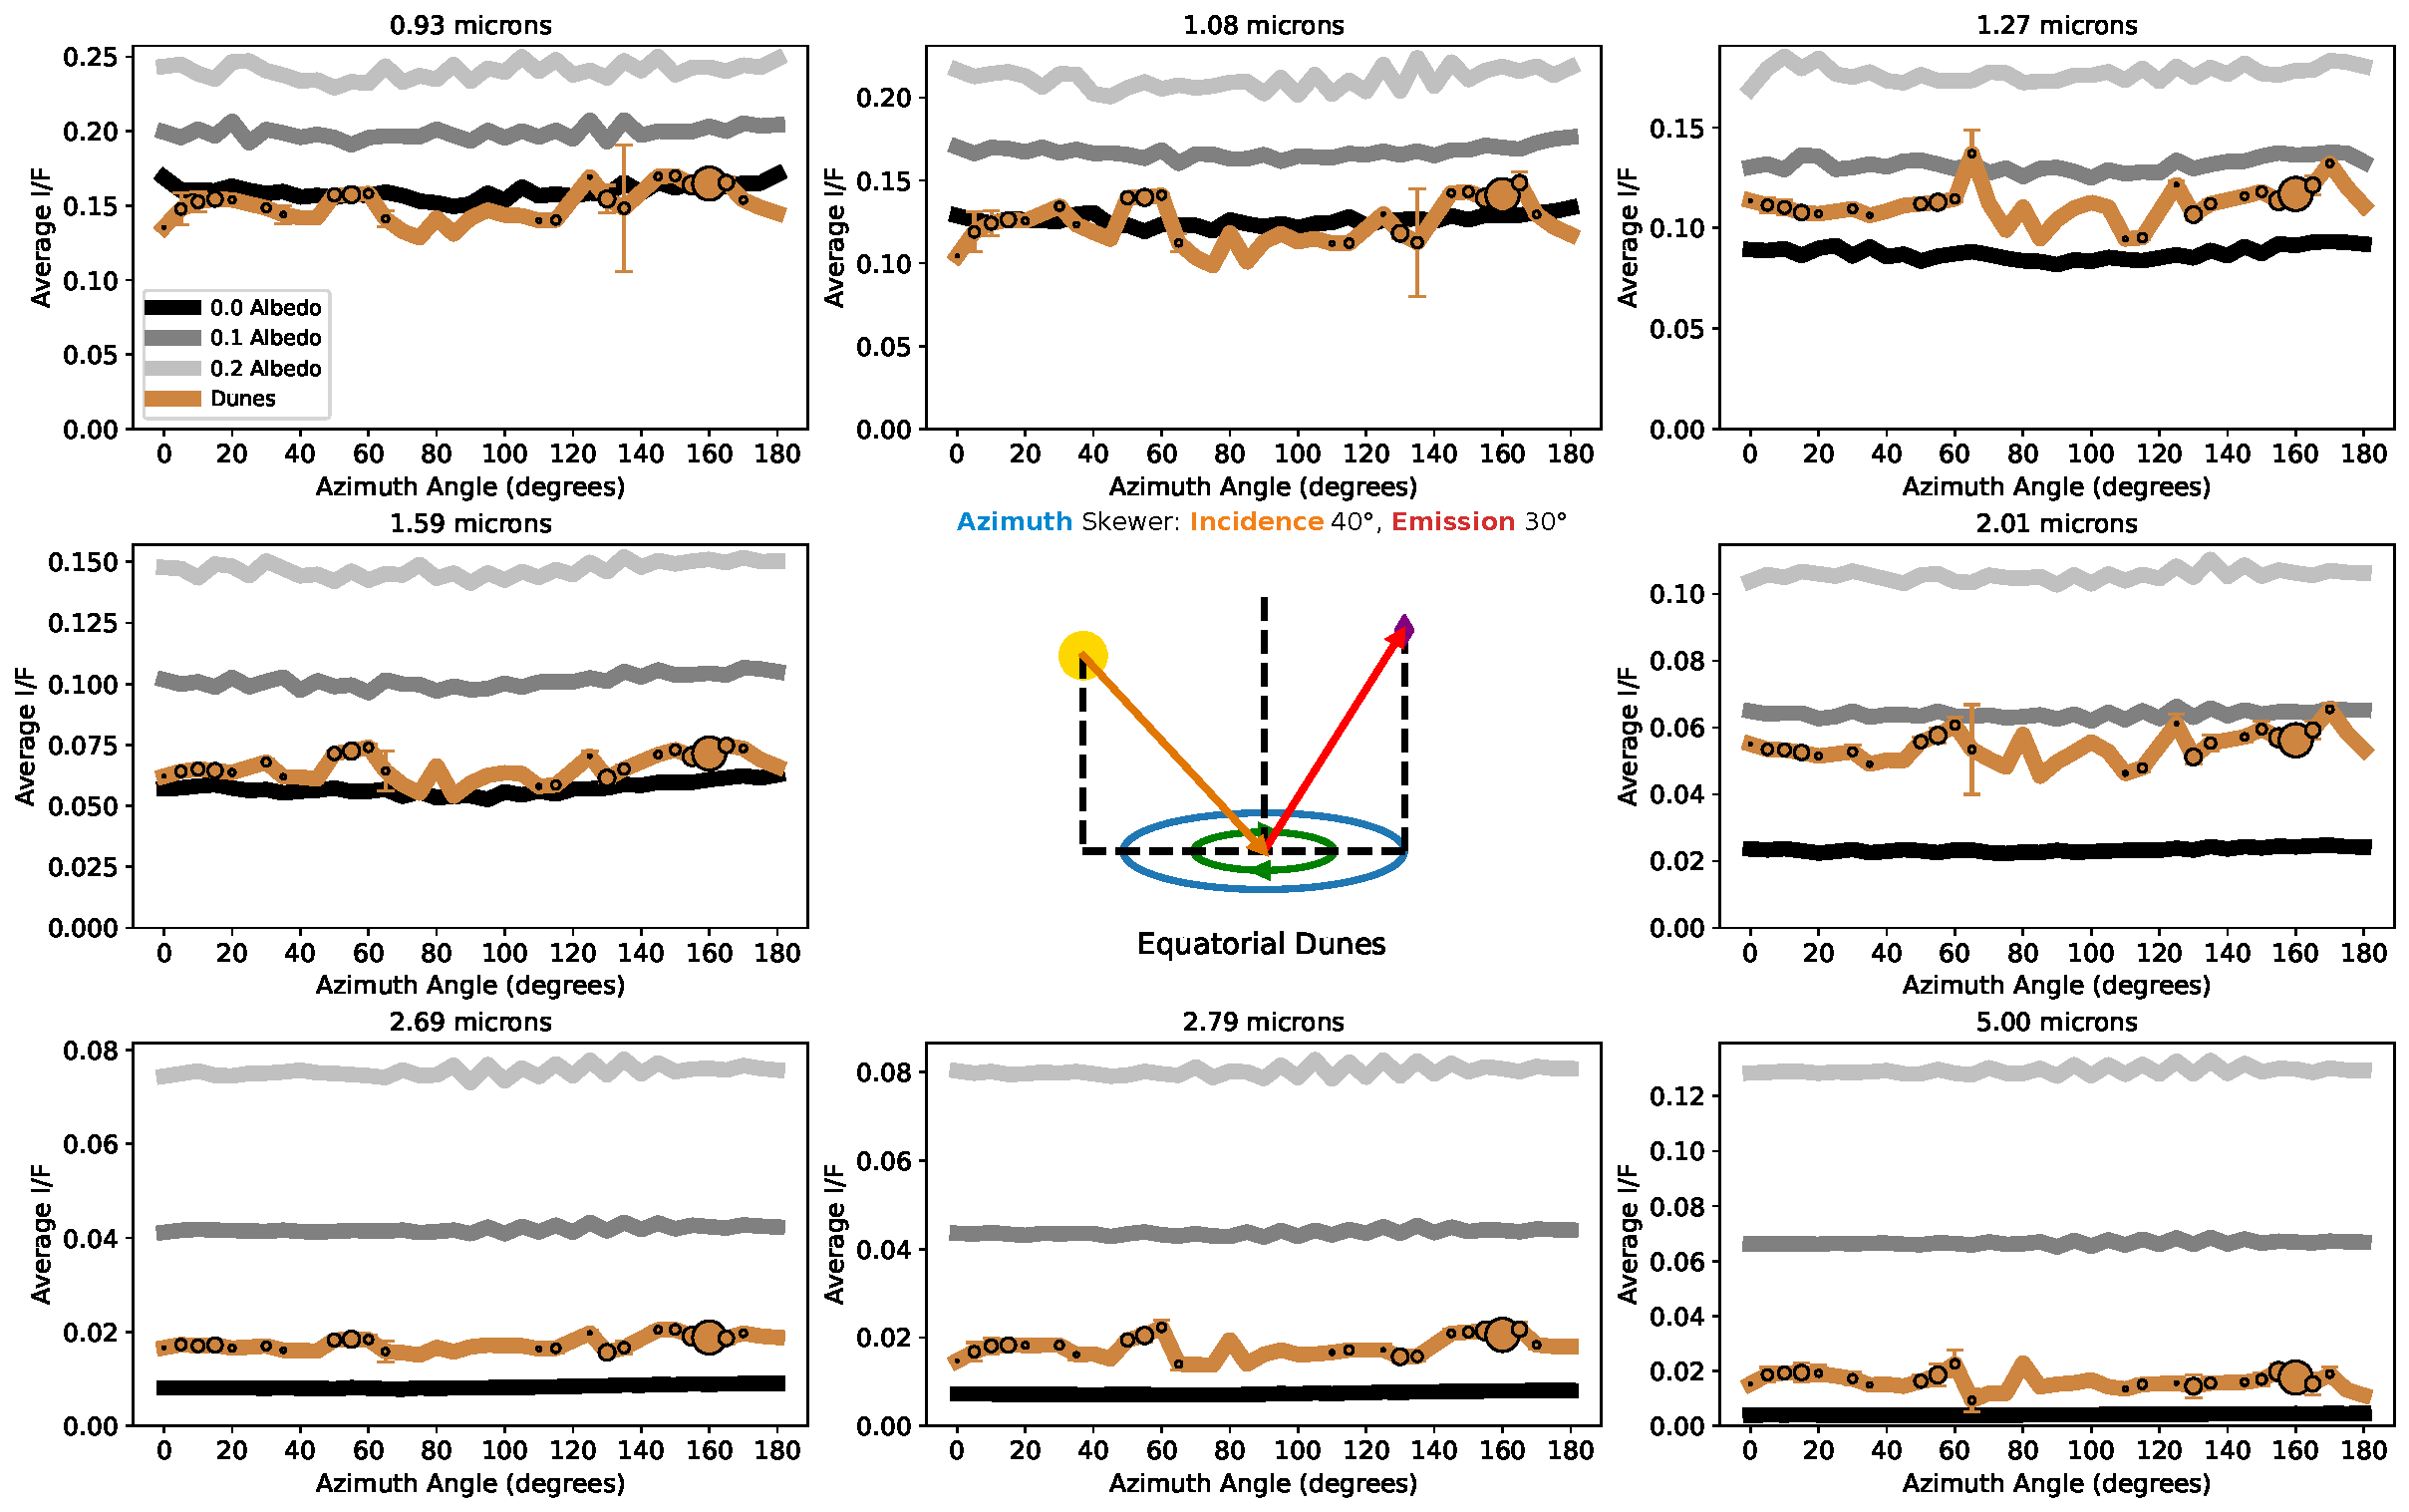
\includegraphics[scale = 0.4]{BrightAzimuthSkewer.pdf}

\centering

\caption{Average I/F azimuth angle skewers for the equatorial dunes with incidence angle fixed at 40$^{\circ}$ and emission angle at 30$^{\circ}$. All eight wavelengths are arranged from shortest to longest, starting from the top left corner. Simulation lines are monochromatic, and the equatorial dunes data are brown. Bins with direct dunes observations have dots plotted over the lines, with larger dots indicating more observations. Segments on the dunes lines without dots are interpolated values. Error bars are made from each noninterpolated bin's standard deviation; most errors are too small to be seen. Note that the vertical axis scale is different for each wavelength. The central area is occupied by a geometry diagram illustrating the specific geometry bins considered for these skewers. All considered azimuth angles are represented by a green circle that coincides with the blue circle representing the surface. The orange and red vectors depict the incidence and emission angles, respectively.}

\label{fig:dunesazimskewer}

\end{figure*}

In addition, since we have data covering a large range of viewing geometries, generating two-dimensional slices of the data becomes viable. In such plots, we still desire to make a direct comparison between reality and simulation, and so in creating Figures \ref{fig:D1}-\ref{fig:D3}, we do not plot I/F, but instead retrieved surface albedo. All three of the figures plot a retrieved sufrace albedo for every emission and azimuth angle with valid observaitons at a single specified incidence angle and IR window wavelength. Figure \ref{fig:D1} is at 55$^{\circ}$ incidence for 1.27 $\mu$m, Figure \ref{fig:D2} is at 50$^{\circ}$ incidence for 2.01 $\mu$m, and Figure \ref{fig:D3} is at 35$^{\circ}$ incidence for 5.00 $\mu$m. 

\begin{figure*}[htbp]

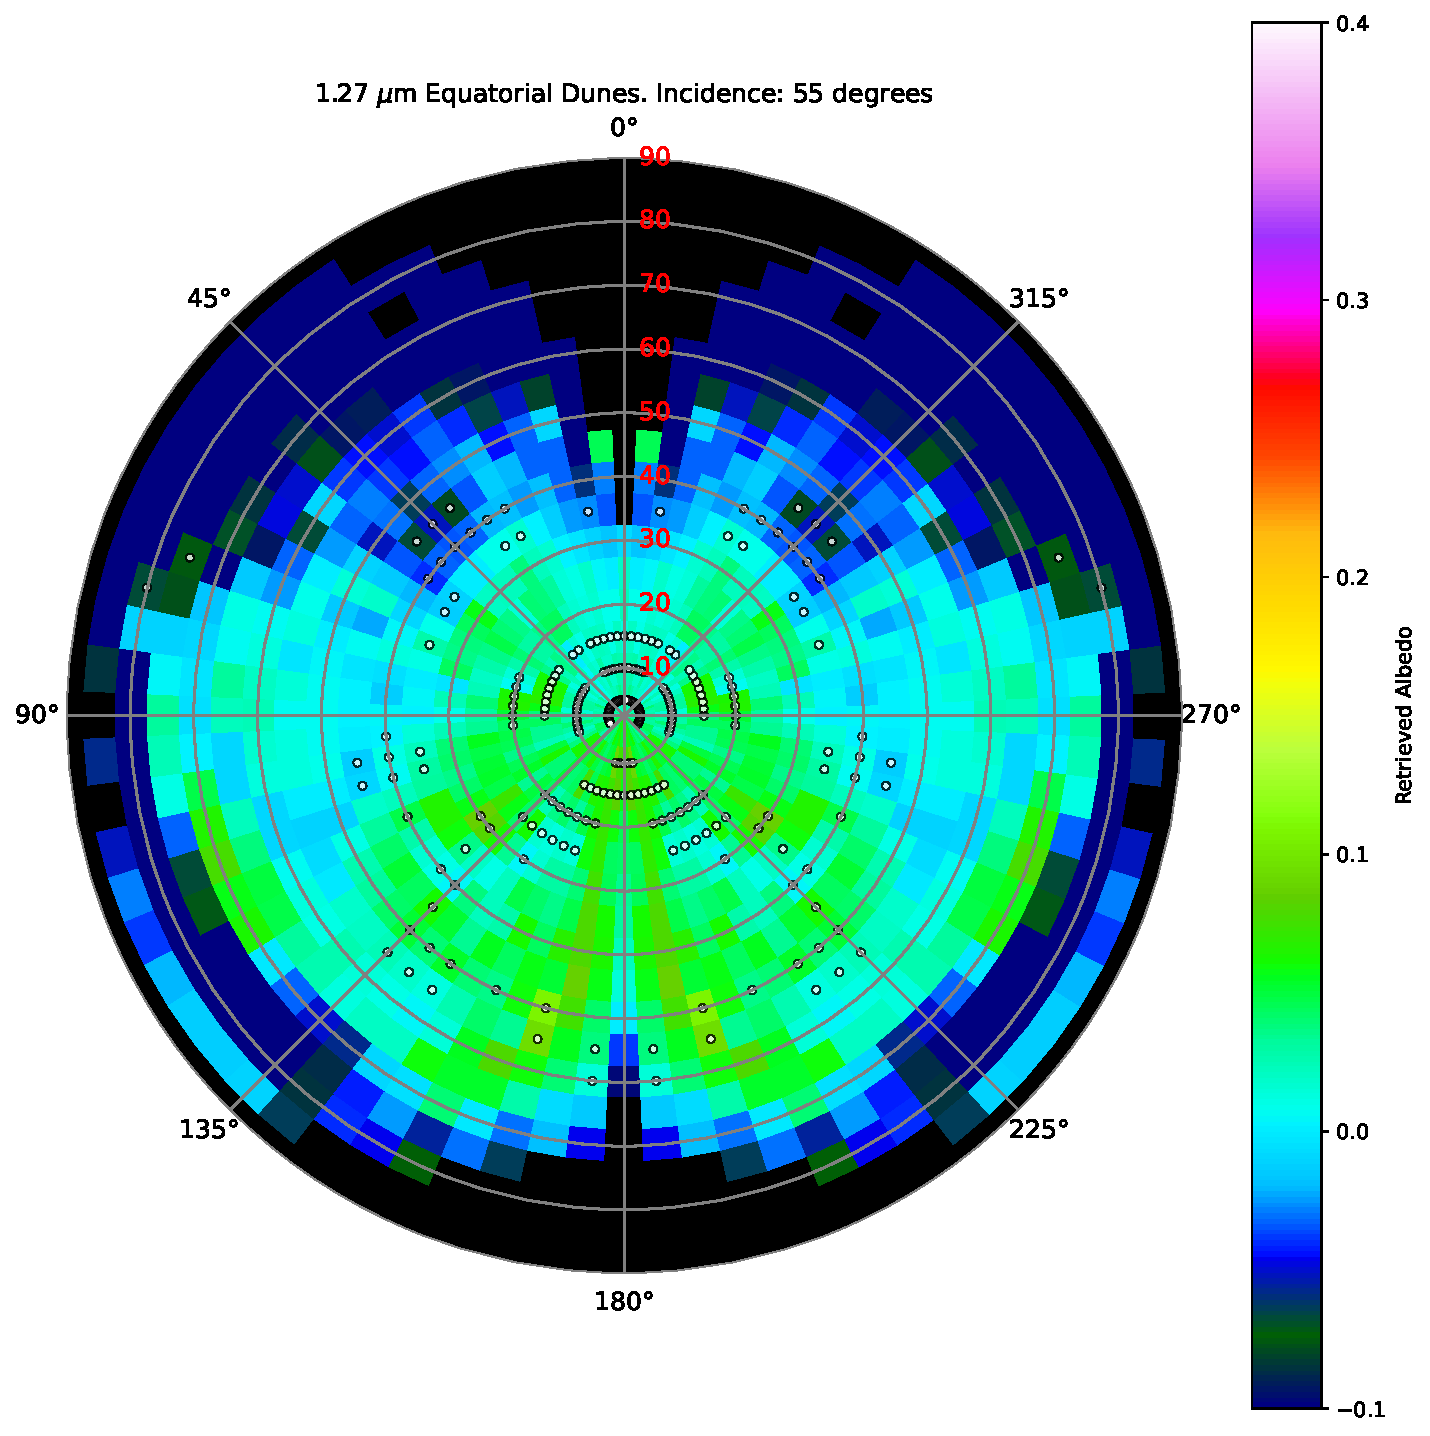
\includegraphics[scale = 0.7]{1.27umDome.pdf}

\centering

\caption{Retrieved surface albedo slice for the 1.27 $\mu$m window dunes at 55$^{\circ}$ incidence angle. The radial coordinate is the emission angle, while the other coordinate is the azimuth angle. The top of the circle is more forward-scattering viewing geometries, while the bottom is more backscattering; sunlight comes in from below. White points represent viewing geometries with real observations; everything else is interpolated or, if black, missing. The plot is mirrored across the central line to fill the bins at azimuths greater than 180$^{\circ}$. Retrieved albedos less than -0.1 and greater than 0.4 are truncated to those values. This particular view showcases the overall lowering of retrieved albedo with increasing emission.}

\label{fig:D1}

\end{figure*}

\begin{figure*}[htbp]

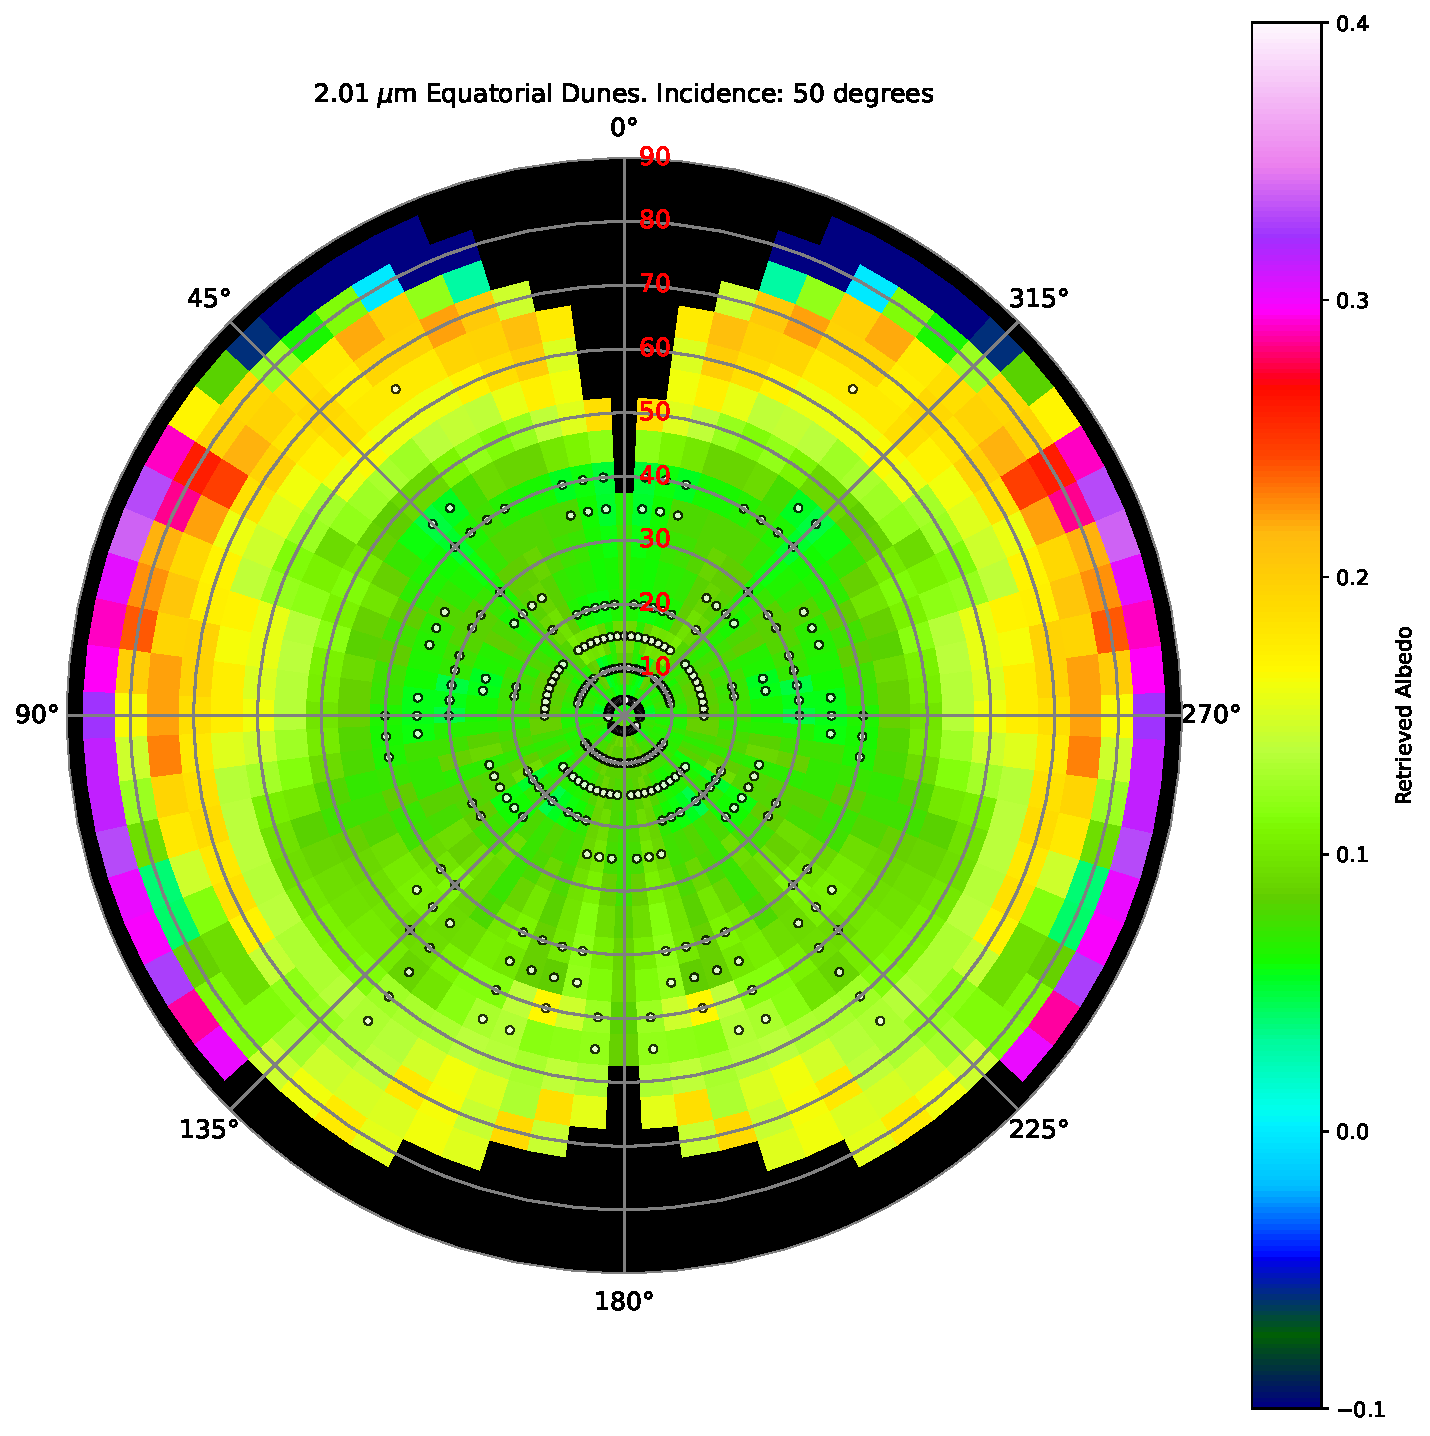
\includegraphics[scale = 0.7]{2.01umDome.pdf}

\centering

\caption{Retrieved surface albedo slice for the 2.01 $\mu$m window dunes at 50$^{\circ}$ incidence angle. The radial coordinate is the emission angle, while the other coordinate is the azimuth angle. The top of the circle is more forward-scattering viewing geometries, while the bottom is more backscattering; sunlight comes in from below. White points represent viewing geometries with real observations; everything else is interpolated or, if black, missing. The plot is mirrored across the central line to fill the bins at azimuths greater than 180$^{\circ}$. Retrieved albedos less than -0.1 and greater than 0.4 are truncated to those values. This particular view showcases the overall increasing of retrieved albedo with increasing emission.}

\label{fig:D2}

\end{figure*}

\begin{figure*}[htbp]

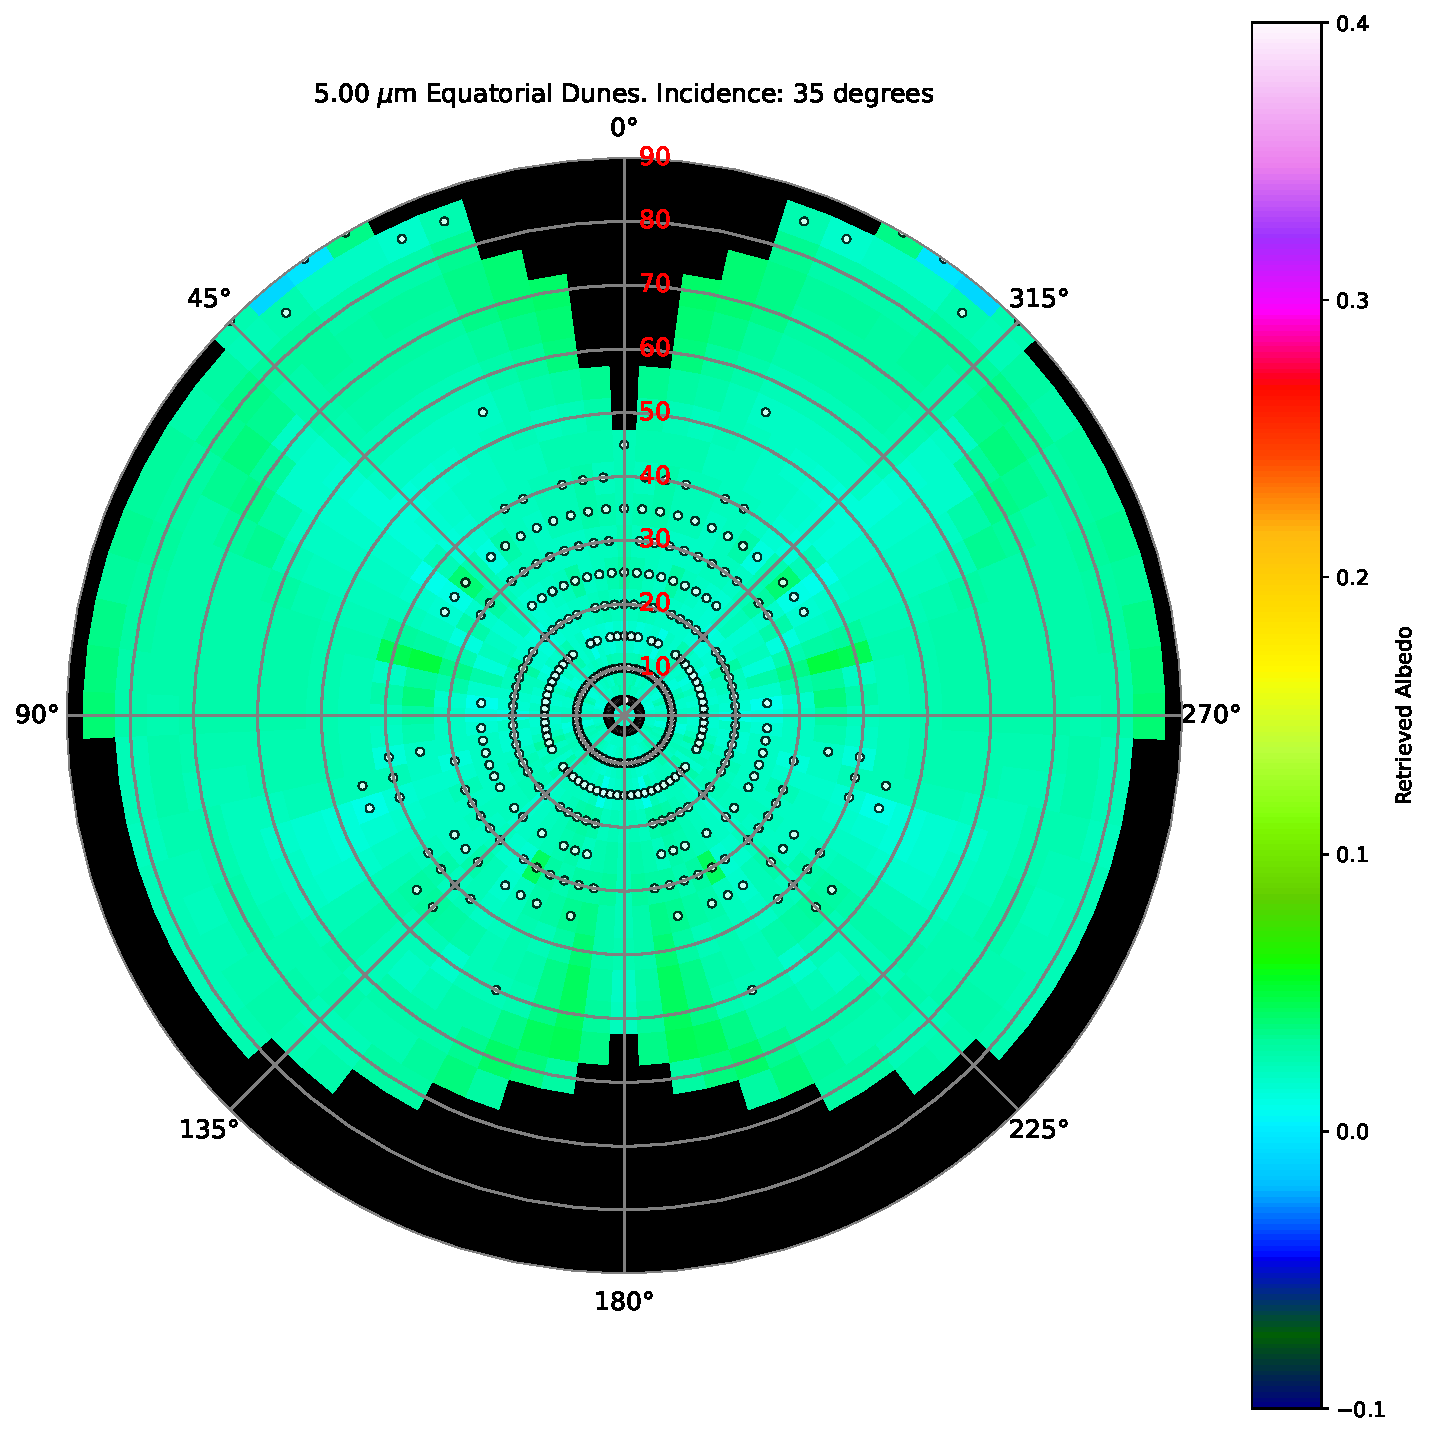
\includegraphics[scale = 0.7]{5umDome.pdf}

\centering

\caption{Retrieved surface albedo slice for the 5.00 $\mu$m window dunes at 35$^{\circ}$ incidence angle. The radial coordinate is the emission angle, while the other coordinate is the azimuth angle. The top of the circle is more forward-scattering viewing geometries, while the bottom is more backscattering; sunlight comes in from below. White points represent viewing geometries with real observations; everything else is interpolated or, if black, missing. The plot is mirrored across the central line to fill the bins at azimuths greater than 180$^{\circ}$. Retrieved albedos less than -0.1 and greater than 0.4 are truncated to those values. This particular view showcases a relatively even retrieved albedo around 0.025.}

\label{fig:D3}

\end{figure*}

To retrieve the surface albedo, we make use of the three different albedos at which the simulations are run: 0.0, 0.1, and 0.2. When the equatorial dunes data point lies between these points, we linearly interpolate to obtain an albedo value for the dunes' surface, and if the real data point is below the 0.0 albedo simulation or above the 0.2 albedo simulation, we extrapolate using a linear "polynomial" fit to retrieve the albedo. This sometimes creates unphysical negative retrieved albedos. We keep these negative values, so when plotted, some indication remains of how far below the predicted 0.0 albedo simulation the real dunes lie.

Examining the results, we find that the dunes data match the shape of the simulations rather closely in the incidence skewer views, as is visible in the skewers of Figure \ref{fig:dunesinciskewer} at 5$^{\circ}$ emission and 50$^{\circ}$ azimuth. Incidence angles higher than 80$^{\circ}$ should be taken with a grain of salt, as Cassini acquired few sufficient observations near and beyond the terminator. That said, the few points that do exist here match the simulated results well. When we examine the full set of data, we do see some minor deviations in incidence skewers at high emission and high azimuth, but there are few observations in those geometries, so the anomaly (if it's even real) is hard to draw conclusions from.

The incidence skewers also clearly show a physical impossibility that sometimes crops up: multiple observations for 0.93 and 1.08 $\mu$m dip below the 0.0 albedo simulation, resulting in a negative retrieved albedo. This retrieval occurs somewhat regularly within the shorter wavelength windows. Figure \ref{fig:D1}, a slice taken at 55$^{\circ}$ incidence, shows quite a few negative retrieved albedos in the 1.27 $\mu$m window. This is particularly disturbing since we expected the interdunes to brighten what we saw in the dunes observations!

Now, in some cases, the negative retrieved albedo occurs because the surface ceases to have a significant result on the simulations: at 100$^{\circ}$ incidence, the simulations might as well be identical and atmospherically-dominated, forcing an unrealistic extrapolation. This happens at high emission angle as well, though to a lesser extent. Unfortunately, this does not explain every negative albedo, as the slice at 55$^{\circ}$ incidence and 1.27 $\mu$m in Figure \ref{fig:D1} shows many negative albedos all over the place, and we have clear examples of observations falling below the dimmest simulation in many skewers.

The physically impossible retrieved albedos may be because SRTC++ does not account for Rayleigh scattering, which is most relevant at short wavelengths \citep{EsSayeh2023}, where negative albedos are most often retrieved. Intuitively, one would expect adding Rayleigh scattering to make the simulation brighter, not dimmer, but subtle effects could be at play--to fully answer this question, we would have to implement Rayleigh scattering, which is on the list for future improvements to SRTC++.

It is notable that in the 1.27 $\mu$m, 55$^{\circ}$ incidence angle slice of Figure \ref{fig:D1}, the negative retrieved albedos cluster largely around the edge of the plot. Indeed, the plot as a whole shows a lowering of retrieved albedo with higher emission angle. We found this behavior in the data for the 0.93, 1.08, and 1.59 $\mu$m windows as well. This lowering of retrieved albedo with emission should not be the case: ideally, for a Lambertian surface, the retrieved albedo would be relatively constant, barring extreme situations where the simulations start overlapping. Such an ideal case can be seen in most 5 $\mu$m albedo retrievals, including our selection at 35$^{\circ}$ incidence in Figure \ref{fig:D3}. 5 $\mu$m is the only one of the eight windows which produces largely consistent albedo retrievals, and it is the window with the least atmospheric influence.

If we examine the other remaining windows (2.01, 2.69, and 2.79 $\mu$m), we find results akin to our selection at 2.01 $\mu$m, 50$^{\circ}$ incidence in Figure \ref{fig:D2}, where the retrieved albedo increases at higher emission angles. This effect is particularly easy to notice in the emission skewers such as the 75$^{\circ}$ incidence and 175$^{\circ}$ azimuth set in Figure \ref{fig:dunesemisskewer}.

Up to around 40$^{\circ}$ emission, the dunes data match the simulations decently well, though the 75$^{\circ}$ incidence and 175$^{\circ}$ azimuth skewers in Figure \ref{fig:dunesemisskewer} continue to demonstrate I/F values below the 0.0 surface albedo simulation at short wavelengths.

At emission angles past 40$^{\circ}$, the simulations are no longer consistent with the data. The 0.93 - 1.59 $\mu$m windows dip further below the 0.0 albedo simulation as emission increases, while 2.01 - 2.79 $\mu$m do the opposite and sharply tick above the simulations. As we can see in Figure \ref{fig:D1} at 1.27$\mu$m, 55$^{\circ}$ incidence and Figure \ref{fig:D2} at 2.01 $\mu$m, 50$^{\circ}$ incidence, this effect is largely azimuthally independent, though the exact degree of the anomaly is adjusted at forward or backscattering directions.

So, how can we explain the variability in retrieved abledo across the various emission angles? There are three primary explanations: biased or contaminated data, real non-Lambertian surface properties, or the atmospheric model not accurately accounting for some effect.

Biased or contaminated data can be ruled out rather quickly: the rise in retrieved surface albedo with emission exists in a wide variety of observations and viewing geometries, occurring at most azimuths. To check further, we divide the restricted BRDFs up based on the time of the observation, finding that the retrieved albedo still deviates with emission across the entire Cassini mission. Separating the data by latitude doesn't remove the effect either, and neither does a longitudinal separation via specific dune fields. There is no bias in time or location on Titan that we can find. Furthermore, the observations that create the rising retrieved albedo are spread out (though there are more in certain times/places than others). Thus, we safely rule out biased or contaminated data.

The second explanation for the rising retrieved albedo is that we're seeing a true non-Lambertian effect from the surface. However, this seems unlikely, as the brightening effect appears azimuthally agnostic: no matter what azimuth we point at, the emission effect exists where we have enough data to see it, and a forward-scattering or backscattering effect would be focused at 0$^{\circ}$ or 180$^{\circ}$, not present everywhere. Topography-oriented explanations also seem unlikely, since the effect begins around 40$^{\circ}$ and only extreme emission angles should be greatly influenced by topography. Not to mention the fact that Titan is rather smooth, topographically speaking, with only a couple of km elevation variation on the surface \citep{Corlies2017}.

That said, we cannot entirely rule out the possibility of true non-Lambertian effects, for it is possible that the material of the dunes behaves in a completely unexpected manner. If we can rule out all other options, we would be forced to consider an unexpected surface property, which would be investigated in future work by testing out various non-Lambertian BRDFs for the surface in the SRTC++ simulations and observing if any of them led to azimuthally agnostic effects.

Lastly, we consider that the model may not accurately account for some atmospheric effect at high emission. While we mentioned Rayleigh scattering earlier, that will only have an important effect on short wavelengths \citep{EsSayeh2023}. We identify three potential places in the atmospheric model where the deficiency could lie: the haze density, the atmospheric single scattering albedo (SSA), or the scattering phase function itself.

The haze density and single scattering albedo theories are easy enough to test by running simulations that modify those parameters. We do exactly that in Figure \ref{fig:hazeSSAtests}, altering the haze to 0.5 and 2.0 density, while adjusting the SSA by factors of 0.8 and 1.2. Since we are only examining 2 $\mu$m here, which has SSA values of around 0.7, the factor of 1.2 won't create unphysical SSA values larger than 1. Unfortunately, none of the adjusted models came close to fixing the issue. 0.5 haze added a strange hump at low emission, 2.0 haze didn't change much, and 0.8 SSA flattened out the curve. 1.2 SSA actually shows a potentially correct slope at higher emission, but at lower emission, it fails completely!

\begin{figure*}[htbp]

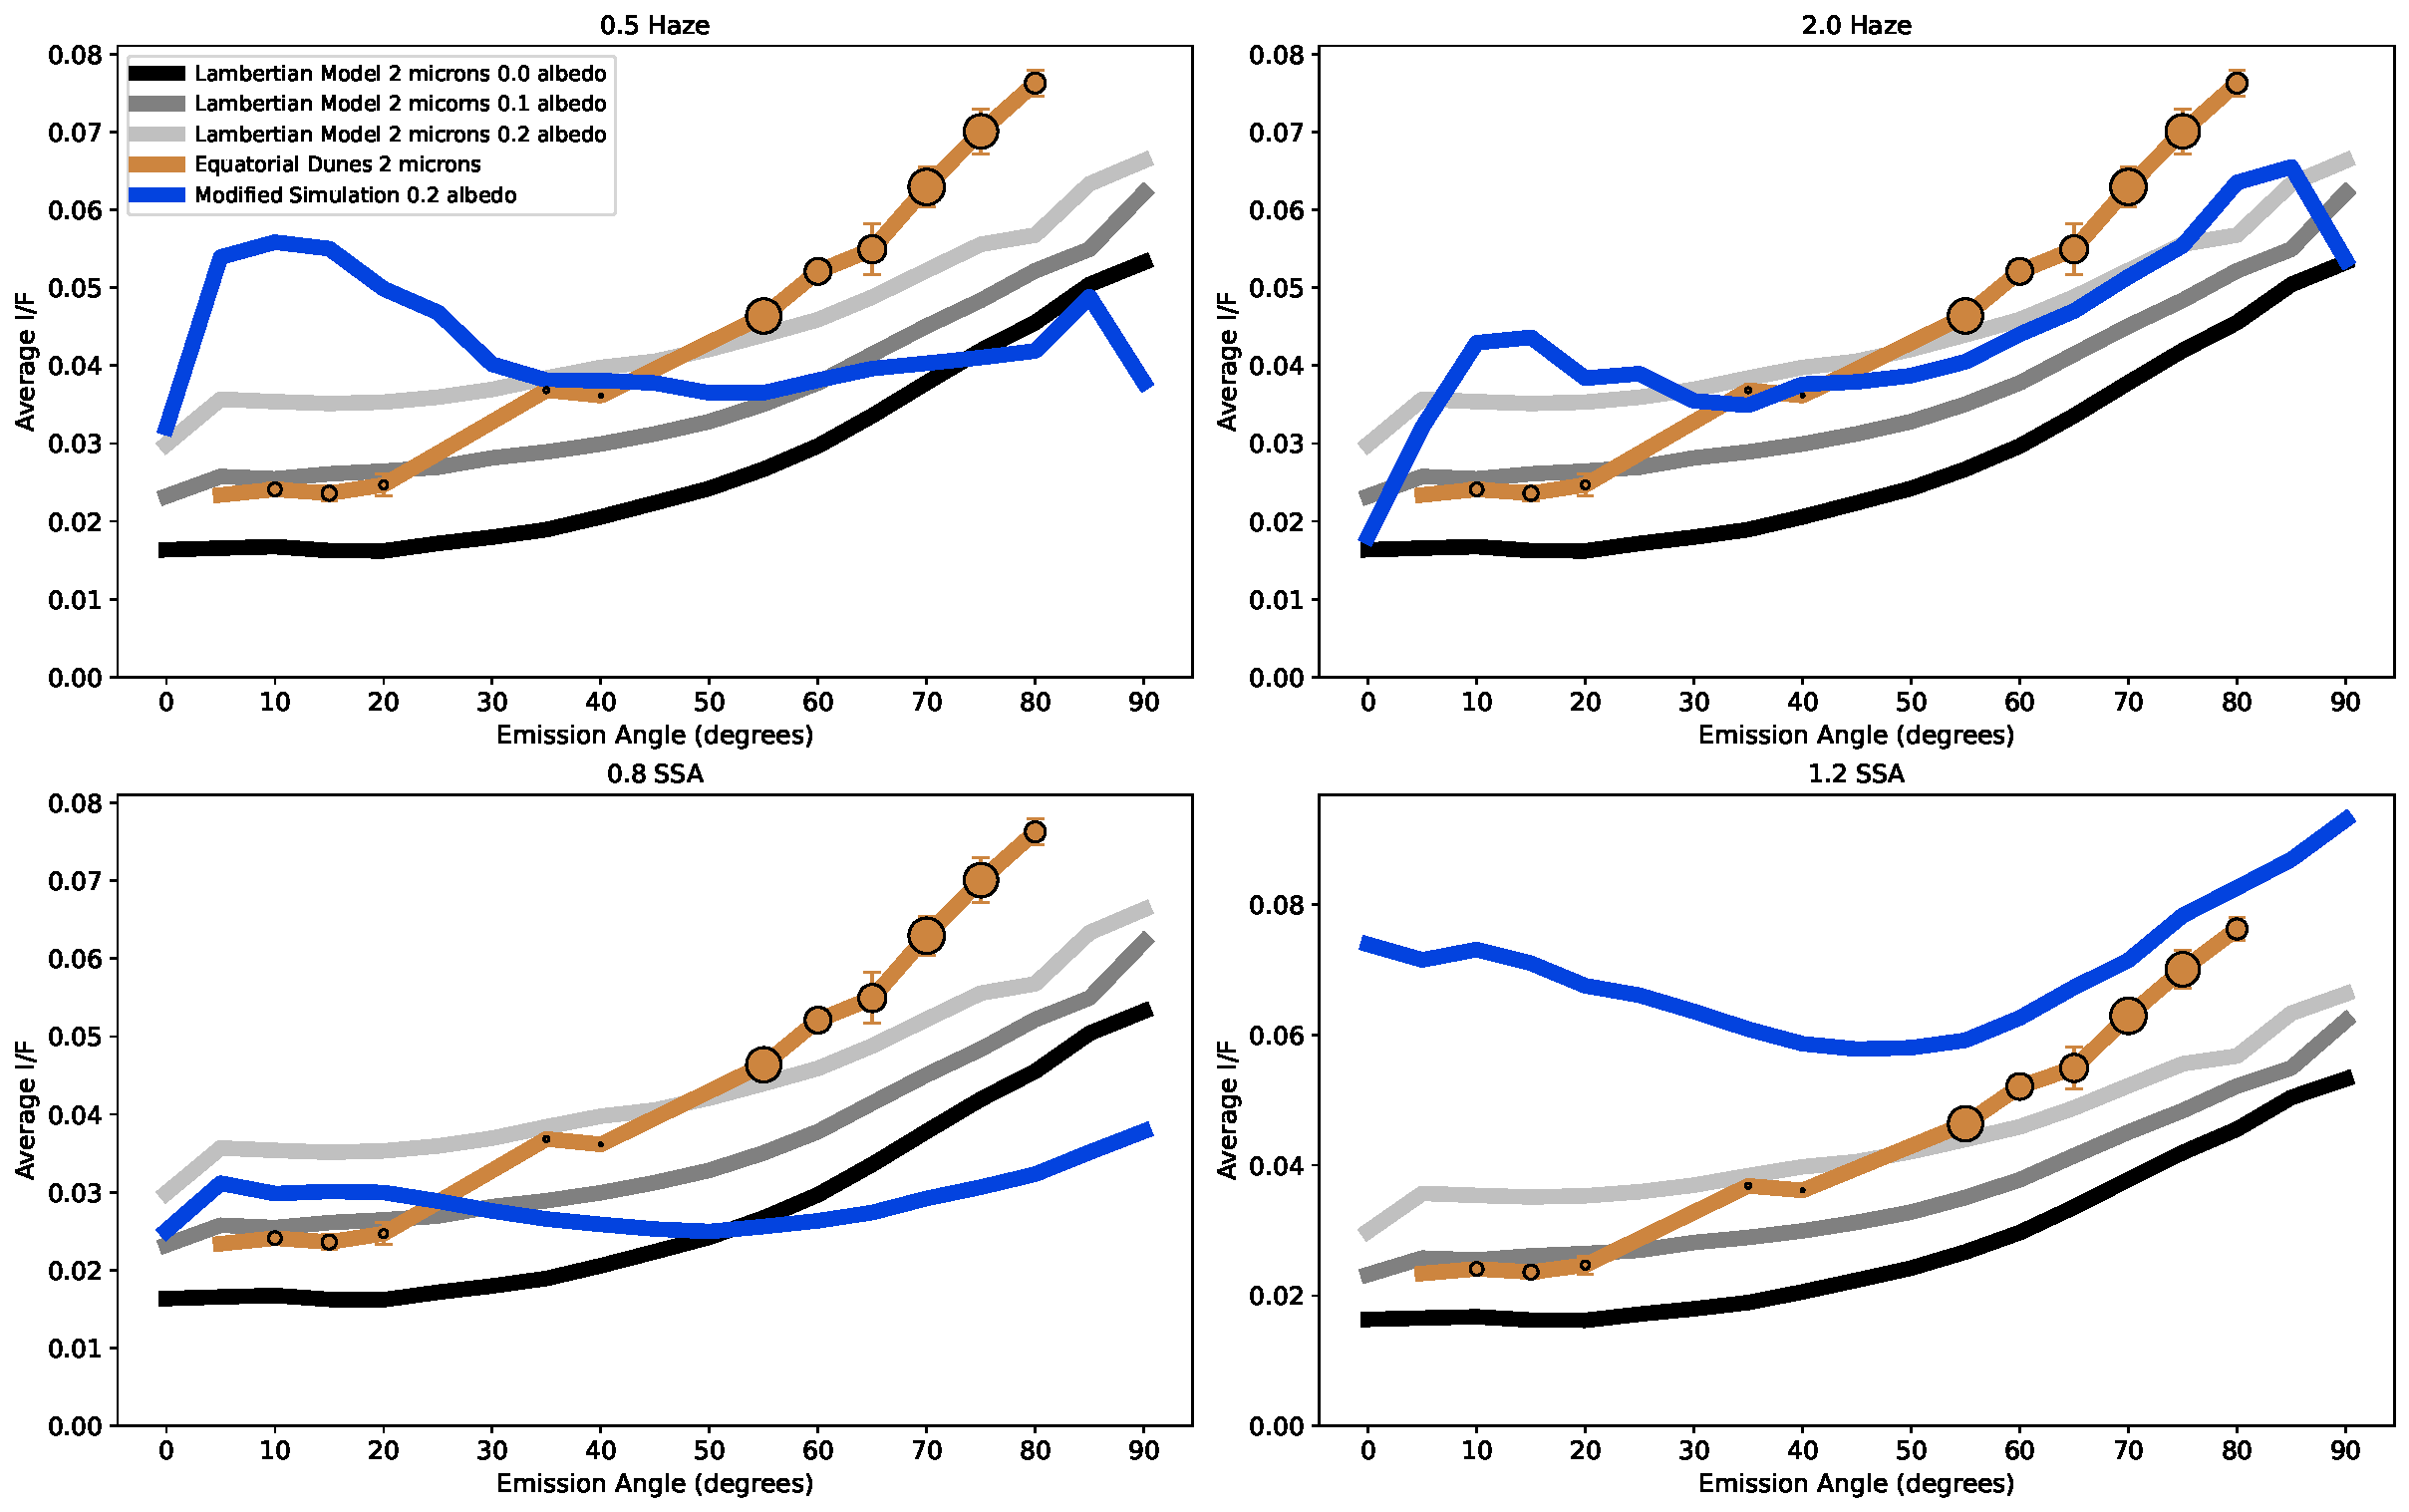
\includegraphics[scale = 0.4]{fourTests.pdf}

\centering

\caption{Emission skewer showcases of altered haze and atmospheric single scattering albedo (SSA) simulations at 2 $\mu$m with fixed 75$^{\circ}$ incidence angle and 175$^{\circ}$ azimuth angle. The viewing geometry is identical to that of Figure \ref{fig:dunesemisskewer}. The monochromatic lines are the unaltered simulations at various albedos, while the brown line is the real dunes data. Error bars are made from each bin's standard deviation for noninterpolated bins. The monochromatic and brown lines are identical in all four displays; the blue lines differ and are simulations run at 0.2 surface albedo with some atmospheric property adjusted. The top left is 0.5 haze density, the top right is double the haze density. The bottom left is SSA dimmed by a factor of 0.8, while the bottom right is SSA brightened by 1.2. Notably, none of the adjustments produce the kind of change that would scale to match the shape of the real dunes data.}

\label{fig:hazeSSAtests}

\end{figure*}

This leads us to the unfortunate conclusion that the likely source of the discrepancy lies in the atmospheric scattering phase function itself. Unlike the other possibilities, testing this is not a simple matter of increasing and decreasing some parameter: the phase function has a wide variety of shapes it could take, and any adjustments to it would need to be normalized. Exploration of the influences of altering the phase function is beyond the scope of this paper, so we leave the full analysis of this question to future work.

Despite the clear deviation at high emission, overall, the simulation and dunes data still match remarkably well. The shape of the dunes data matches the incidence and azimuth skewer predictions, even if sometimes it sits below the 0.0 albedo simulation. Azimuth skewers in particular are well behaved, with most being clearly flat in the dunes data, such as in the skewers at 40$^{\circ}$ incidence and 30$^{\circ}$ emission in Figure \ref{fig:dunesazimskewer}.

As a final, more quantitative, check on validation, we turn to compare our retrieved surface albedos with those reported for the dunes in prior literature \citep{McCord2006, Bonnefoy2016, Solomonidou2018, Brossier2018, EsSayeh2023}. In order to come up with a singular retrieved albedo value, we consider every bin that contains real observations, ignoring interpolated values. Each bin is sorted by wavelength and then combined into a single data set, which is then plotted as a violin plot in Figure \ref{fig:albedosContext}. We select the median of the data as our overall retrieved albedo and obtain uncertainties from the median absolute deviation (MAD) times 1.4826.

\begin{figure*}[htbp]

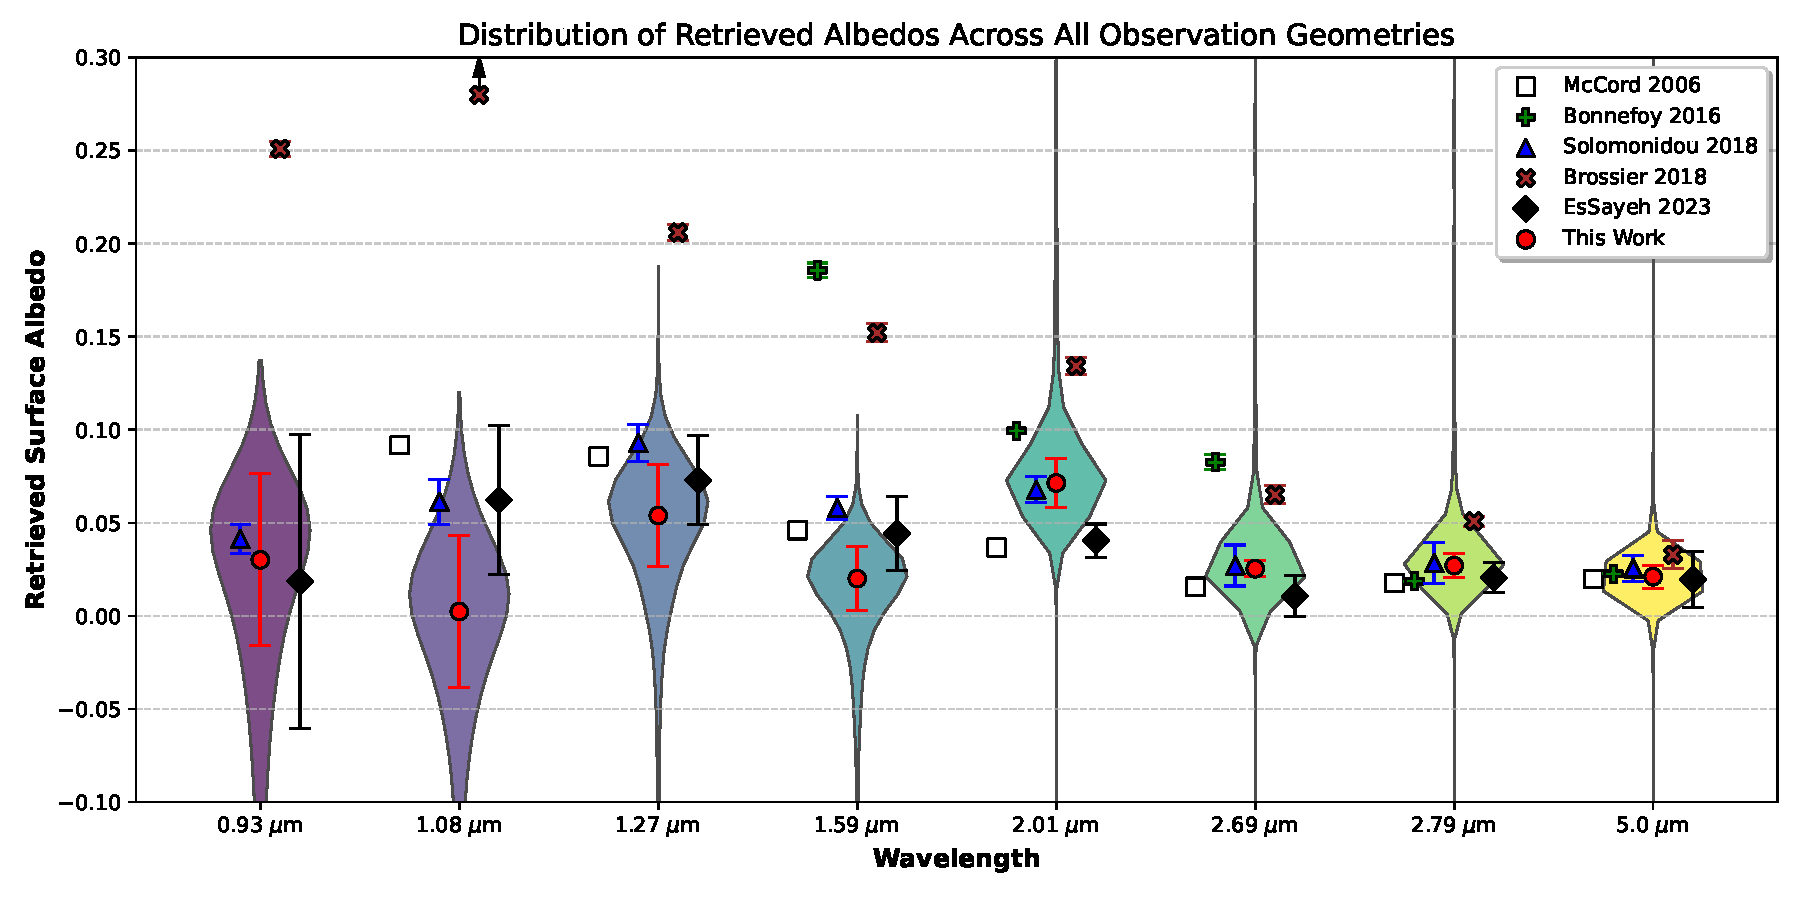
\includegraphics[scale = 0.6]{Albedo_Violin_Plots_Context.pdf}

\centering

\caption{Retrieved surface albedo violin distribution plots compared with retrieved surface albedos of prior studies. These violin plots consider retrieved albedos made at all viable observation angles. The red points are the medians of our retrieved surface albedos, while our error bars are median absolute deviations (MAD) times 1.4826. Other error bars are what the indicated source reported. \cite{McCord2006} is the only source without reported uncertainties or error bars; all other points from previous work have them, though in many cases they are too small to be seen. \cite{Brossier2018} reports their values as surface single scattering albedos, which are converted to Lambertian surface albedos via procedures outlined in \cite{Hapke2012}. \cite{Brossier2018} has a single point at 1.08 $\mu$m that is off the scale; we saw no reason to compress the horizontal axis even further to fit it into the frame, considering how far it is from all other sources for the same window. If no point is plotted for a source, that source did not report an albedo value for that window.}

\label{fig:albedosContext}

\end{figure*}

As we have reason to suspect our methods are unreliable at extreme viewing geometries, we also create a second version of Figure \ref{fig:albedosContext} where we only consider incidence and emission angles of 40$^{\circ}$ or less, as that is where we identified the emission angle discrepancy beginning. Those results are in Figure \ref{fig:albedosContextSmol} and create a somewhat different set of medians. We present the numerical values of the medians and modified MAD values in Table \ref{table:theTable}.

\begin{figure*}[htbp]

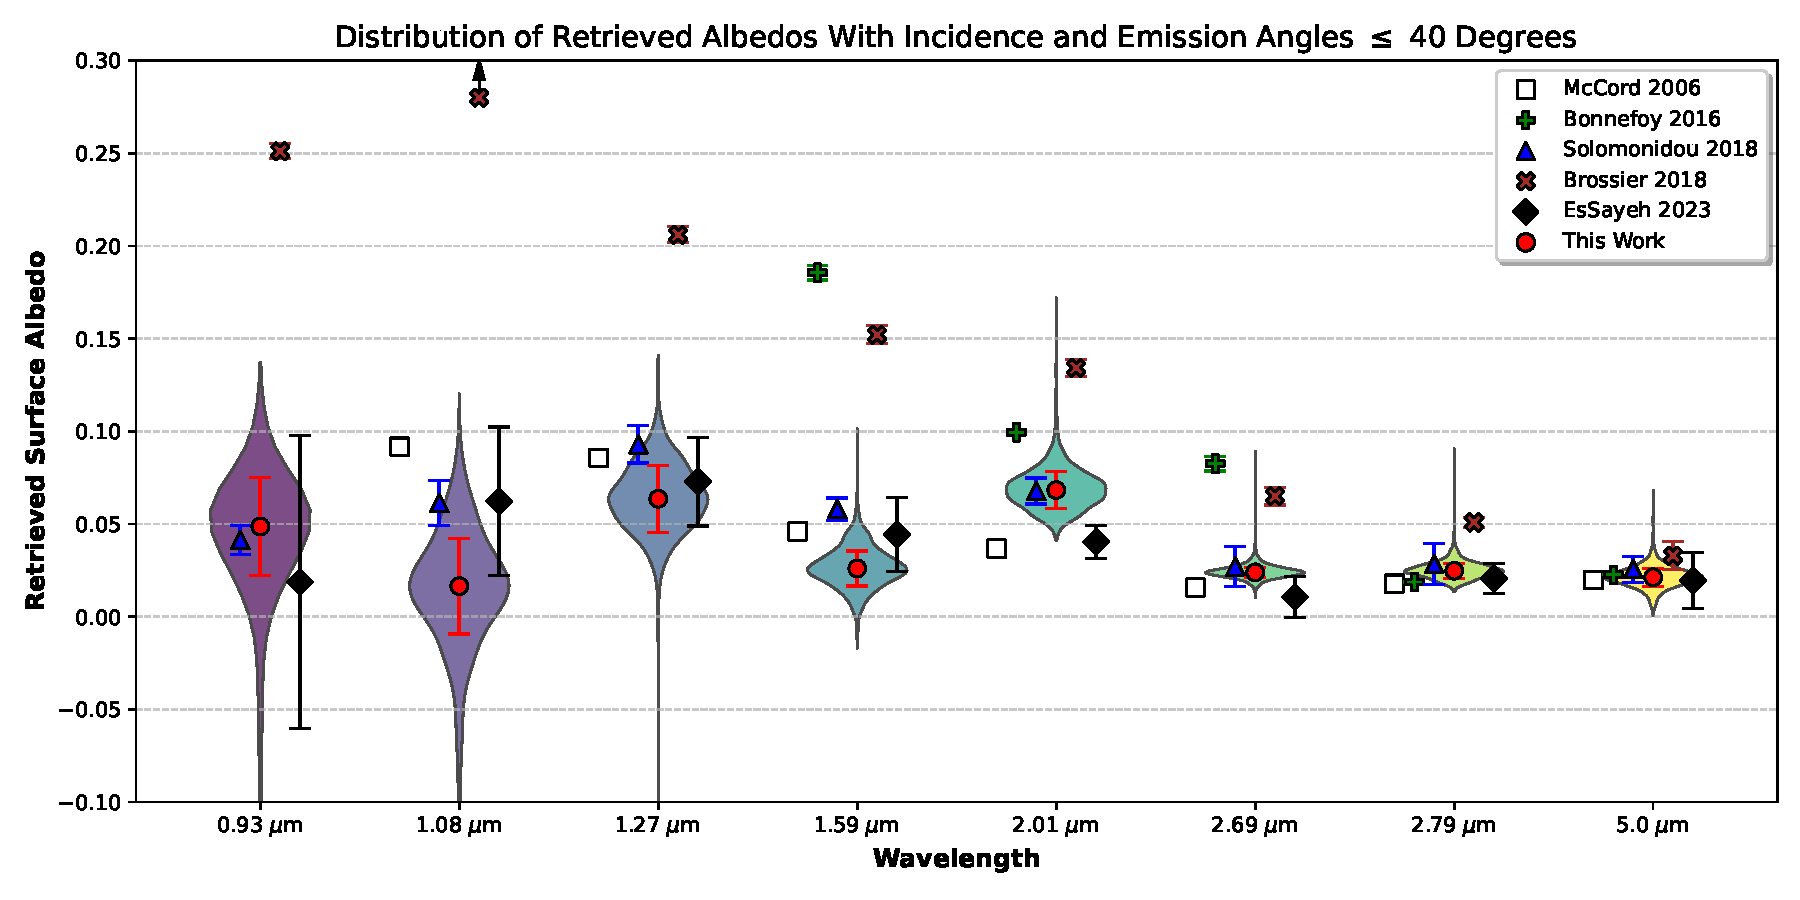
\includegraphics[scale = 0.6]{Albedo_Violin_Plots_Context_Smol.pdf}

\centering

\caption{Retrieved surface albedo violin distribution plots compared with retrieved surface albedos of prior studies. These violin plots only consider retrieved albedos at incidence and emission angles lower than 40$^{\circ}$. The red points are the medians of our retrieved surface albedos, while our error bars are median absolute deviations (MAD) times 1.4826. Other error bars are what the indicated source reported. \cite{McCord2006} is the only source without reported uncertainties or error bars; all other points from previous work have them, though in many cases they are too small to be seen. \cite{Brossier2018} reports their values as surface single scattering albedos, which are converted to Lambertian surface albedos via procedures outlined in \cite{Hapke2012}. \cite{Brossier2018} has a single point at 1.08 $\mu$m that is off the scale; we saw no reason to compress the horizontal axis even further to fit it into the frame, considering how far it is from all other sources for the same window. If no point is plotted for a source, that source did not report an albedo value for that window.}

\label{fig:albedosContextSmol}

\end{figure*}

\begin{table*}[htbp]

\centering

\begin{tabular}{ccc}

\multicolumn{3}{c}{Retrieved Albedos} \\

Wavelength & Full Retrieved Albedo & Truncated Retrieved Albedo \\

\hline

0.93 $\mu$m & 0.030$\pm$0.031 & 0.049$\pm$0.018 \\

\hline

1.08 $\mu$m & 0.002$\pm$0.027 & 0.017$\pm$0.017 \\

\hline

1.27 $\mu$m & 0.054$\pm$0.019 & 0.064$\pm$0.012 \\

\hline

1.59 $\mu$m & 0.020$\pm$0.012 & 0.026$\pm$0.006 \\

\hline

2.01 $\mu$m & 0.071$\pm$0.009 & 0.068$\pm$0.007 \\

\hline

2.69 $\mu$m & 0.025$\pm$0.003 & 0.024$\pm$0.002 \\

\hline

2.79 $\mu$m & 0.027$\pm$0.004 & 0.025$\pm$0.003 \\

\hline

5.00 $\mu$m & 0.021$\pm$0.004 & 0.021$\pm$0.003 \\

\hline

\end{tabular}

\caption{Table of retrieved albedos for all eight IR wavelength windows. The "full" retrieved albedos consider real observations at all angles, the "truncated" retrieved albedos only consider incidence and emission angles of 40$^{\circ}$ or less. The values themselves are the medians, and the uncertainties are given by the median absolute deviation (MAD) times 1.4826.}

\label{table:theTable}

\end{table*}

In both the full and limited data sets, our retrieval for 5.00 $\mu$m is consistent with all previous work. The double windows 2.69 and 2.79 $\mu$m show good agreement as well, though already at this point we can see prior work diverging into two separate camps: \cite{McCord2006, Solomonidou2018, EsSayeh2023}, and our work on one side, \cite{Bonnefoy2016} and \cite{Brossier2018} on the other. We are unsure why there should be such drastic differences between these retrievals, especially considering the fact that \cite{Solomonidou2018} and \cite{Brossier2018} use the same radiative transfer model! \textbf{\color{red}Currently doing research on this, it's clear the answer to why they are different will not be simple. It may have something to do with the ambiguity of what "albedo" refers to, or interpretations therein. Alternatively, they could be making a correction that the others are not. Rayleigh scattering?\color{black}}

Leaving aside the brighter \cite{Bonnefoy2016} and \cite{Brossier2018} points for a moment, our results show general agreement that only improves upon ignoring all incidence and emission angles beyond 40$^{\circ}$ in Figure \ref{fig:albedosContextSmol}. The primary exception is 1.08 $\mu$m, which we identified as having poor correlation with our simulations before. We are currently unsure why 1.08 $\mu$m in particular is poorly retrieved--we would expect both it and 0.93 $\mu$m to be similarly affected by atmospheric contamination noise and Rayleigh Scattering. Yet our 0.93 $\mu$m retrieval agrees with both \cite{McCord2006} and \cite{EsSayeh2023}.

We recognize the irony in throwing out larger incidence and emission angles when the extreme angles were precisely why we chose SRTC++ as our radiative transfer model in the first place. However, had we not used a spherical model for Titan, we would never have identified the model deficiency at high emission. 

In general, our retrievals are either in line with previous predictions of darker dunes or slightly dimmer than them, the exception being 2.00 $\mu$m, which is slightly brighter in our predictions, if anything. The small wavelength windows show the least certainty and have the most physically impossible albedo retrievals, evidenced by the lower part of the distributions dipping significantly into the negative.

Given the relative agreement our retrieved albedos have with three different sources, we have reason to believe our simulation results are reasonable. Though, noting the wide spread of results across multiple studies, we are forced to conclude that the community's knowledge of Titan's surface albedo is limited and likely to change as new techniques are developed and analyses performed.

In the end, where do these simulation and observation comparisons leave us? With the shapes of the dunes data matching the restricted BRDFs so closely in incidence and azimuth, it seems reasonable to conclude that the dunes act substantially as a Lambertian surface. The primary evidence for non-Lambertian behavior comes from the inconsistent albedo retrieval at variable emission, which does not appear to have an azimuthal dependence and is likely an atmospheric effect not accounted for in the simulation, rather than a true non-Lambertian effect.

However, we recognize that our method of binning spectels together and averaging them all makes us significantly less sensitive to dramatic changes over tiny angular extents, such as the sharp central peak often seen in the opposition effect, sometimes less than one degree away from opposition \citep{Kulyk2008, Schaefer2008}. It is worthwhile to perform a more focused check for such an effect.

We perform a direct search across our entire database, cube by cube, for an opposition effect in the dunes (or an equivalent effect in the forward-scattering direction). We find no signs of any such effect. For seven of the eight windows, this is to be expected: the opposition effect is all but removed by diffuse lighting and indirect viewing angles via scattering \citep{Schroder2008}. However, the 5 $\mu$m window would not be subject to this limitation as it sees significant unimpeded sunlight even when it is near sunset \citep{Barnes2018b}. Even here, we find no evidence of an opposition effect.

To be fair, the closest any observation we consider gets to opposition is between 1 and 2 degrees. This does not rule out a narrow and sharp opposition effect, as these can be confined to within 0.1$^{\circ}$ \citep{Kulyk2008, Schaefer2008}. The solar disc's footprint on Titan is around 0.05 $\deg$ \citep{Barnes2011}, further implying it would not be detectable.Huygens observed the opposition effect spike to begin around 0.2$^{\circ}$ \citep{Karkoschka2012}, and the observation was made with Huygens' own illumination, not the sun's. Furthermore, Huygens did not land on the dunes. 

The viewing geometry to definitively confirm or deny the opposition effect does not exist in the Cassini VIMS data for the dunes; we can only say that if the dunes have an opposition effect, it is a narrow one with little-to-no broad component.

We also find no pseudo-specular forward-scattering component in the dunes, even though we did find an observation that approached zero degrees from the specular direction. We, admittedly, did not expect to see a forward-scattering effect in the first place, as we did for the opposition effect.

\section{Summary and Conclusion} \label{sec:conclusion}

There are two primary purposes to this paper: to constrain Titan's surface dune properties and to validate the SRTC++ simulations against real data.

On the validation front, SRTC++ in general calculates restricted BRDF trends that match the real data in incidence and azimuth angles, but clearly doesn’t always produce the correct albedo, as evidenced by situations where the recovered albedo is below 0.0, an impossibility. As these moments primarily occur at short wavelengths, the impossible albedos could be the influence of Rayleigh scattering. Alternatively, or perhaps additionally, its source could be a fault in the characterization of atmospheric haze--the far more prevalent observed deviations with increasing emission angle imply there's something missing there.

More quantitatively, our general retrieved albedos for the dunes in each of the individual windows are largely consistent with previous work, with the exception of the 1.08 $\mu$m window, which is significantly lower. We have no explanation for why 1.08 $\mu$m specifically is an issue; we would expect it to be just as unreliable as 0.93 $\mu$m, but this is clearly not the case. We are also unclear as to the reason there appear to be two different trends in retrieved surface albedos for the dunes across the literature. Our results corroborate the lower albedo values rather than the higher albedo values.

Despite these caveats, SRTC++ still produces smooth lines parallel to the real data in most incidence and azimuth skewers, only with inconsistent surface albedo retrieval. As such, the simulations are still useful for characterizing Titan's surface, particularly looking for clear deviations from the Lambertian assumption. It is telling, then, that we found almost none. There is no evidence of an opposition effect and no evidence for a forward scattering component to the surface BRDF. The only major deviation is the dimming and brightening some windows exhibit at high emission angles--but, again, we think that it is more likely a model insufficiency than a real effect. The Huygens landing site also shows Lambertian behavior, though we do not say this with certainty, considering the limited nature of the observations at that location.

Our ultimate conclusion is that Titan's dunes are Lambertian surfaces, or very close to it. This result is not unexpected, for Earth's sand is also generally Lambertian \citep{Hapke1963}, though Earth's sand exhibits an opposition effect within two degrees of zero phase angle \citep{Wise2022}, which would have been detectable were this the case on Titan. However, it is thought that the width of an opposition effect narrows the further an object is from the sun \citep{Karkoschka2012} due to the smaller angular diameter of the solar disk, so we cannot say that we should have seen an opposition effect on the dunes. Furthermore, Earth's sand and Titan's dunes are characteristically different, as most of Earth's deserts are quite bright, while Titan's dunes are the darkest solid terrain on its surface.

Future work would include improving SRTC++ to simulate the atmosphere properly at high emission--or, if that were to prove impossible, investigating what other effects might cause the inaccuracies. If we cannot track down a specific issue with SRTC++ through this investigation, we will investigate unusual surface BRDFs (ones without atmospheric contributions). The hope is that one of them will produce an azimuthally agnostic effect with rising emission when seen through the atmosphere.

This work could also be turned to the specular lakes at Titan's north pole; while the atmosphere is not as well characterized there, we can use the relatively simple lake surface phase functions to probe where exactly it's poorly characterized. Other terrain types on Titan could also be examined--it would just require a more manual rather than automated approach, as the other terrains are not as distinct as the dunes. Preliminary investigations on this front have been performed, but none of the other terrains (including the equatorial bright terrain) have results as regular and as expansive as the dunes.

\begin{acknowledgments}

Acknowledgements:

We wish to acknowledge the pyVIMS code \citep{Seignovert2021}, even though we did not end up using it in our final analysis; it was extremely helpful for preliminary investigations and early code.

The restricted BRDFs created for this research are available by request in the form of numpy arrays.

All authors are funded by grant \#80NSSC22K0340 from the NASA Cassini Data Analysis Program.

\end{acknowledgments}

\label{ACK}

\bibliography{Bibliography}{}

\bibliographystyle{aasjournal}

\end{document}